% ******************************* PhD Thesis Template **************************
% Please have a look at the README.md file for info on how to use the template

\documentclass[a4paper,12pt,times,numbered,print,index,abstract]{Classes/PhDThesisPSnPDF}

% ******************************************************************************
% ******************************* Class Options ********************************
% *********************** See README for more details **************************
% ******************************************************************************

% `a4paper'(The University of Cambridge PhD thesis guidelines recommends a page
% size a4 - default option) or `a5paper': A5 Paper size is also allowed as per
% the Cambridge University Engineering Deparment guidelines for PhD thesis
%
% `11pt' or `12pt'(default): Font Size 10pt is NOT recommended by the University
% guidelines
%
% `oneside' or `twoside'(default): Printing double side (twoside) or single
% side.
%
% `print': Use `print' for print version with appropriate margins and page
% layout. Leaving the options field blank will activate Online version.
%
% `index': For index at the end of the thesis
%
% `draft': For draft mode without loading any images (same as draft in book)
%
% `abstract': To generate only the title page and abstract page with
% dissertation title and name, to submit to the Student Registry
%
% `chapter`: This option enables only the specified chapter and it's references
%  Useful for review and corrections.
%
% ************************* Custom Page Margins ********************************
%
% `custommargin`: Use `custommargin' in options to activate custom page margins,
% which can be defined in the preamble.tex. Custom margin will override
% print/online margin setup.
%
% *********************** Choosing the Fonts in Class Options ******************
%
% `times' : Times font with math support. (The Cambridge University guidelines
% recommend using times)
%
% `fourier': Utopia Font with Fourier Math font (Font has to be installed) 
%            It's a free font.
%
% `customfont': Use `customfont' option in the document class and load the
% package in the preamble.tex
%
% default or leave empty: `Latin Modern' font will be loaded.
%
% ********************** Choosing the Bibliography style ***********************
%
% `authoryear': For author-year citation eg., Krishna (2013)
%
% `numbered': (Default Option) For numbered and sorted citation e.g., [1,5,2]
%
% `custombib': Define your own bibliography style in the `preamble.tex' file.
%              `\RequirePackage[square, sort, numbers, authoryear]{natbib}'. 
%              This can be also used to load biblatex instead of natbib 
%              (See Preamble) 
%
% **************************** Choosing the Page Style *************************
%
% `default (leave empty)': For Page Numbers in Header (Left Even, Right Odd) and
% Chapter Name in Header (Right Even) and Section Name (Left Odd). Blank Footer.
%
% `PageStyleI': Chapter Name next & Page Number on Even Side (Left Even).
% Section Name & Page Number in Header on Odd Side (Right Odd). Footer is empty.
%
% `PageStyleII': Chapter Name on Even Side (Left Even) in Header. Section Number
% and Section Name in Header on Odd Side (Right Odd). Page numbering in footer


% ********************************** Preamble **********************************
% Preamble: Contains packages and user-defined commands and settings
% ******************************************************************************
% ****************************** Custom Margin *********************************

% Add `custommargin' in the document class options to use this section
% Set {innerside margin / outerside margin / topmargin / bottom margin}  and
% other page dimensions

\ifsetMargin
\else
    \RequirePackage[left=37mm,right=30mm,top=35mm,bottom=30mm]{geometry}
    \setFancyHdr % To apply fancy header after geometry package is loaded
\fi

% *****************************************************************************
% ******************* Fonts (like different typewriter fonts etc.)*************

% Add `customfont' in the document class option to use this section

\ifsetFont
\else
    % Set your custom font here and use `customfont' in options. Leave empty to
    % load computer modern font (default LaTeX font).  

    \RequirePackage{libertine} 
\fi

% *****************************************************************************
% **************************** Custom Packages ********************************


% ************************* Algorithms and Pseudocode **************************

%\usepackage{algpseudocode} 


% ********************Captions and Hyperreferencing / URL **********************

% Captions: This makes captions of figures use a boldfaced small font. 
%\RequirePackage[small,bf]{caption}

\RequirePackage[labelsep=space,tableposition=top]{caption} 
\renewcommand{\figurename}{Fig.} %to support older versions of captions.sty

% ************************ Formatting / Footnote *******************************

%\usepackage[perpage]{footmisc} %Range of footnote options 


% ****************************** Line Numbers **********************************

%\RequirePackage{lineno}
%\linenumbers

% *************************** Graphics and figures *****************************

%\usepackage{rotating}
%\usepackage{wrapfig}
%\usepackage{float}
\usepackage{subfig} %note: subfig must be included after the `caption` package. 


% ********************************** Table *************************************

%\usepackage{longtable}
%\usepackage{multicol}
%\usepackage{multirow}
%\usepackage{tabularx}


% ***************************** Math and SI Units ******************************

\usepackage{amsfonts}
\usepackage{amsmath}
\usepackage{amssymb}
%\usepackage{siunitx} % use this package module for SI units


% *********************************** Other ***********************************

\usepackage[showboxes, absolute]{textpos}


% *****************************************************************************
% *************************** Bibliography  and References ********************

%\usepackage{cleveref} %Referencing without need to explicitly state fig /table

% Add `custombib' in the document class option to use this section
\ifsetBib % True, Bibliography option is chosen in class options
\else % If custom bibliography style chosen then load bibstyle here

   \RequirePackage[square, sort, numbers, authoryear]{natbib} % CustomBib

% If you would like to use biblatex for your reference management, as opposed to the default `natbibpackage` pass the option `custombib` in the document class. Comment out the previous line to make sure you don't load the natbib package. Uncomment the following lines and specify the location of references.bib file

% \RequirePackage[backend=biber, style=numeric-comp, citestyle=numeric, sorting=nty, natbib=true]{biblatex}
% \bibliography{References/references} %Location of references.bib only for biblatex

\fi


% changes the default name `Bibliography` -> `References'
\renewcommand{\bibname}{References}


% *****************************************************************************
% *************** Changing the Visual Style of Chapter Headings ***************

% Uncomment the section below. Requires titlesec package.

%\RequirePackage{titlesec}
%\newcommand{\PreContentTitleFormat}{\titleformat{\chapter}[display]{\scshape\Large}
%{\Large\filleft{\chaptertitlename} \Huge\thechapter}
%{1ex}{}
%[\vspace{1ex}\titlerule]}
%\newcommand{\ContentTitleFormat}{\titleformat{\chapter}[display]{\scshape\huge}
%{\Large\filleft{\chaptertitlename} \Huge\thechapter}{1ex}
%{\titlerule\vspace{1ex}\filright}
%[\vspace{1ex}\titlerule]}
%\newcommand{\PostContentTitleFormat}{\PreContentTitleFormat}
%\PreContentTitleFormat


% ******************************************************************************
% ************************* User Defined Commands ******************************
% ******************************************************************************

% *********** To change the name of Table of Contents / LOF and LOT ************

%\renewcommand{\contentsname}{My Table of Contents}
%\renewcommand{\listfigurename}{My List of Figures}
%\renewcommand{\listtablename}{My List of Tables}


% ********************** TOC depth and numbering depth *************************

\setcounter{secnumdepth}{2}
\setcounter{tocdepth}{2}

% ******************************* Nomenclature *********************************

% To change the name of the Nomenclature section, uncomment the following line

%\renewcommand{\nomname}{Symbols}


% ********************************* Appendix ***********************************

% The default value of both \appendixtocname and \appendixpagename is `Appendices'. These names can all be changed via: 

%\renewcommand{\appendixtocname}{List of appendices}
%\renewcommand{\appendixname}{Appndx}


% ************************ Thesis Information & Meta-data **********************
% Thesis title and author information, refernce file for biblatex
% ************************ Thesis Information & Meta-data **********************
%% The title of the thesis
\title{Low cost imaging and image processing with the Raspberry Pi} 
%\texorpdfstring is used for PDF metadata. Usage:
%\texorpdfstring{LaTeX_Version}{PDF Version (non-latex)} eg.,
%\texorpdfstring{$sigma$}{sigma}

%% The full name of the author
\author{Jamie Magee}

%% Department (eg. Department of Engineering, Maths, Physics)
\dept{Department of Engineering}

%% University and Crest
\university{University of Cambridge}
\crest{
\includegraphics[width=0.25\textwidth]{University_Crest}}

%% You can redefine the submission text:
% Default as per the University guidelines: This dissertation is submitted for
% the degree of Doctor of Philosophy
%\renewcommand{\submissiontext}{change the default text here if needed}

%% Full title of the Degree 
\degree{Master of Engineering}
 
%% College affiliation (optional)
\college{Gonville and Caius College}

%% Submission date
\degreedate{2014} 

%% Meta information
\subject{LaTeX} \keywords{{LaTeX} {PhD Thesis} {Engineering} {University of
Cambridge}}



% ***************************** Abstract Separate ****************************** 
% To printout only the titlepage and the abstract with the PhD title and the 
% author name for submission to the Student Registry, use the `abstract' option in
% the document class. 

\ifdefineAbstract
 \pagestyle{empty}
 \includeonly{Declaration/declaration, Abstract/abstract} 
\fi

% ***************************** Chapter Mode ***********************************
% The chapter mode allows user to only print particular chapters with references
% Title, Contents, Frontmatter are disabled by default
% Useful option to review a particular chapter or to send it to supervisior.
% To use choose `chapter' option in the document class

\ifdefineChapter
 \includeonly{Chapter3/chapter3} 
\fi

% ******************************** Front Matter ********************************
\begin{document}

\frontmatter

\begin{titlepage}

\maketitle

\end{titlepage}

%% ******************************* Thesis Dedidcation ********************************

\begin{dedication} 

I would like to dedicate this thesis to my loving parents ...

\end{dedication}


% ******************************* Thesis Declaration ********************************

\begin{declaration}

I hereby declare that, except where specifically indicated, the work submitted herein is my own original work.

% Author and date will be inserted automatically from thesis.tex \author \degreedate

\end{declaration}


%% ************************** Thesis Acknowledgements *****************************

\begin{acknowledgements}      


And I would like to acknowledge ...


\end{acknowledgements}

% ************************** Thesis Abstract *****************************
% Use `abstract' as an option in the document class to print only the titlepage and the abstract.
\begin{abstract}
Optical flow is a critical tool in many experimental methods such as Particle Image Velocimetry for flow analysis and soil mechanics, speckle tracking echocardiography in medical imaging, as well as mechanical testing. It enables data capture from systems in which placing conventional instrumentation can be difficult. During this project Lucas-Kanade, Farnebäck, and SimpleFlow optical flow methods were compared using artificial and real world datasets on the limited hardware of the Raspberry Pi. Obtaining acceptable levels of performance on the embedded system of the Raspberry Pi could reduce the costs of research and teaching involving optical flow methods. For dense optical flow Farnebäck was found to have the lowest processing time, SimpleFlow was found to have the highest accuracy, and Lucas-Kanade was found to lie somewhere in between. However, when using Lucas-Kanade as a sparse algorithm it was found to have the lowest processing time. Instructions, aimed at undergraduate level, on how to install the tools used in this project are provided, along with the robust toolset used in testing. Practical applications were also demonstrated by integrating optical flow methods into a tensile testing machine developed as part of the OpenLabTools initiative. Further work investigating performance under arbitrary affine transformations, or projective transformations using the toolset developed as part of this project is possible. Visualisation of vector field showing the curl or the divergence of the vector field may also be a useful tool. 
\end{abstract}


% *********************** Adding TOC and List of Figures ***********************

\tableofcontents

%\listoffigures

%\listoftables 

% \printnomenclature[space] space can be set as 2.5cm between symbol and
% description
%\printnomencl

% ******************************** Main Matter *********************************
\mainmatter

\chapter{Introduction}

\ifpdf
    \graphicspath{{Section1/Figs/Raster/}{Section1/Figs/PDF/}{Section1/Figs/}}
\else
    \graphicspath{{Section1/Figs/Vector/}{Section1/Figs/}}
\fi

\begin{figure}[htpb]
  \centering
  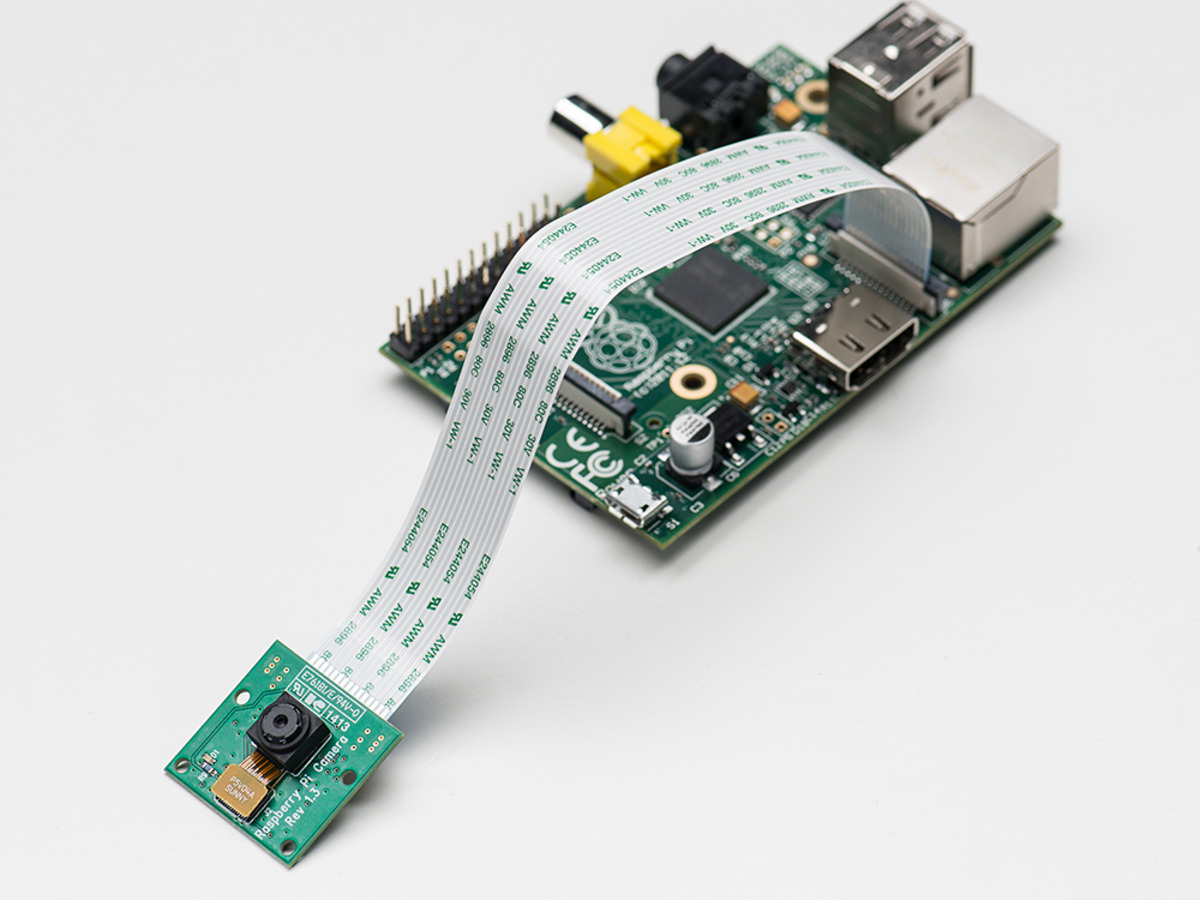
\includegraphics[width=.8\textwidth]{RaspberryPi}
  \caption{Raspberry Pi with camera module attached}
  \label{fig:raspi}
\end{figure}

The Raspberry Pi is a low cost, credit-card sized computer developed in the UK by the Raspberry Pi Foundation. The primary objective of the Raspberry Pi is to increase, and encourage the teaching of computer science in schools. In this regard it has been highly successful and since its launch in February 2012 it has sold over 2 million units~\cite{2mil}, however its success has also been, in part, due to the hobbyist and scientific markets. The Raspberry Pi boasts a 700MHz ARMv6k, 512 MB of RAM and a full Linux operating system for \$35~\cite{Broadcom-BCM2835-Website}. In addition, the Raspberry Pi foundation have released a camera module that supports up to 1080p30 video capture, and can be seen in Figure~\ref{fig:raspi}. All of these features make the Raspberry Pi an ideal candidate for imaging and image processing on a low budget.

Optical flow is the apparent motion of objects in a scene due to relative motion between an observer and the objects being observed as seen in Figure~\ref{fig:opticalflow}. It is a critical tool in many experimental methods such as Particle Image Velocimetry~\cite{quenot1998particle} for flow analysis and and soil mechanics, speckle tracking echocardiography~\cite{speckle} in medical imaging for assessing the contractile performance of cardiac and skeletal muscles, as well as mechanical testing~\cite{harris2012characterizing} for measuring the strain in a sample undergoing a tensile test. The recurring theme in the use of optical flow methods, are that they enable data capture from systems in which placing conventional instrumentation can be difficult or even impossible. There already exist commercial packages for executing optical flow algorithms, however licenses can often be costly and the software can require high end hardware, therefore obtaining acceptable levels of performance on the embedded system of the Raspberry Pi could reduce the costs of research and teaching involving optical flow methods. This project, as part of the OpenLabTools initiative, aims to provide access to optical flow methods on low cost and low powered hardware. The main objectives for the project are to:

\begin{itemize}
  \item Provide access to optical flow methods on cheap and readily available hardware
  \item Perform online and offline processing using the Raspberry Pi
  \item Capture data using the Raspberry Pi Camera
  \item Integrate with existing experiments and other OpenLabTools projects
  \item Provide a clear set of instructions aimed at undergraduate level
\end{itemize}

\begin{figure}[htpb]
  \centering
  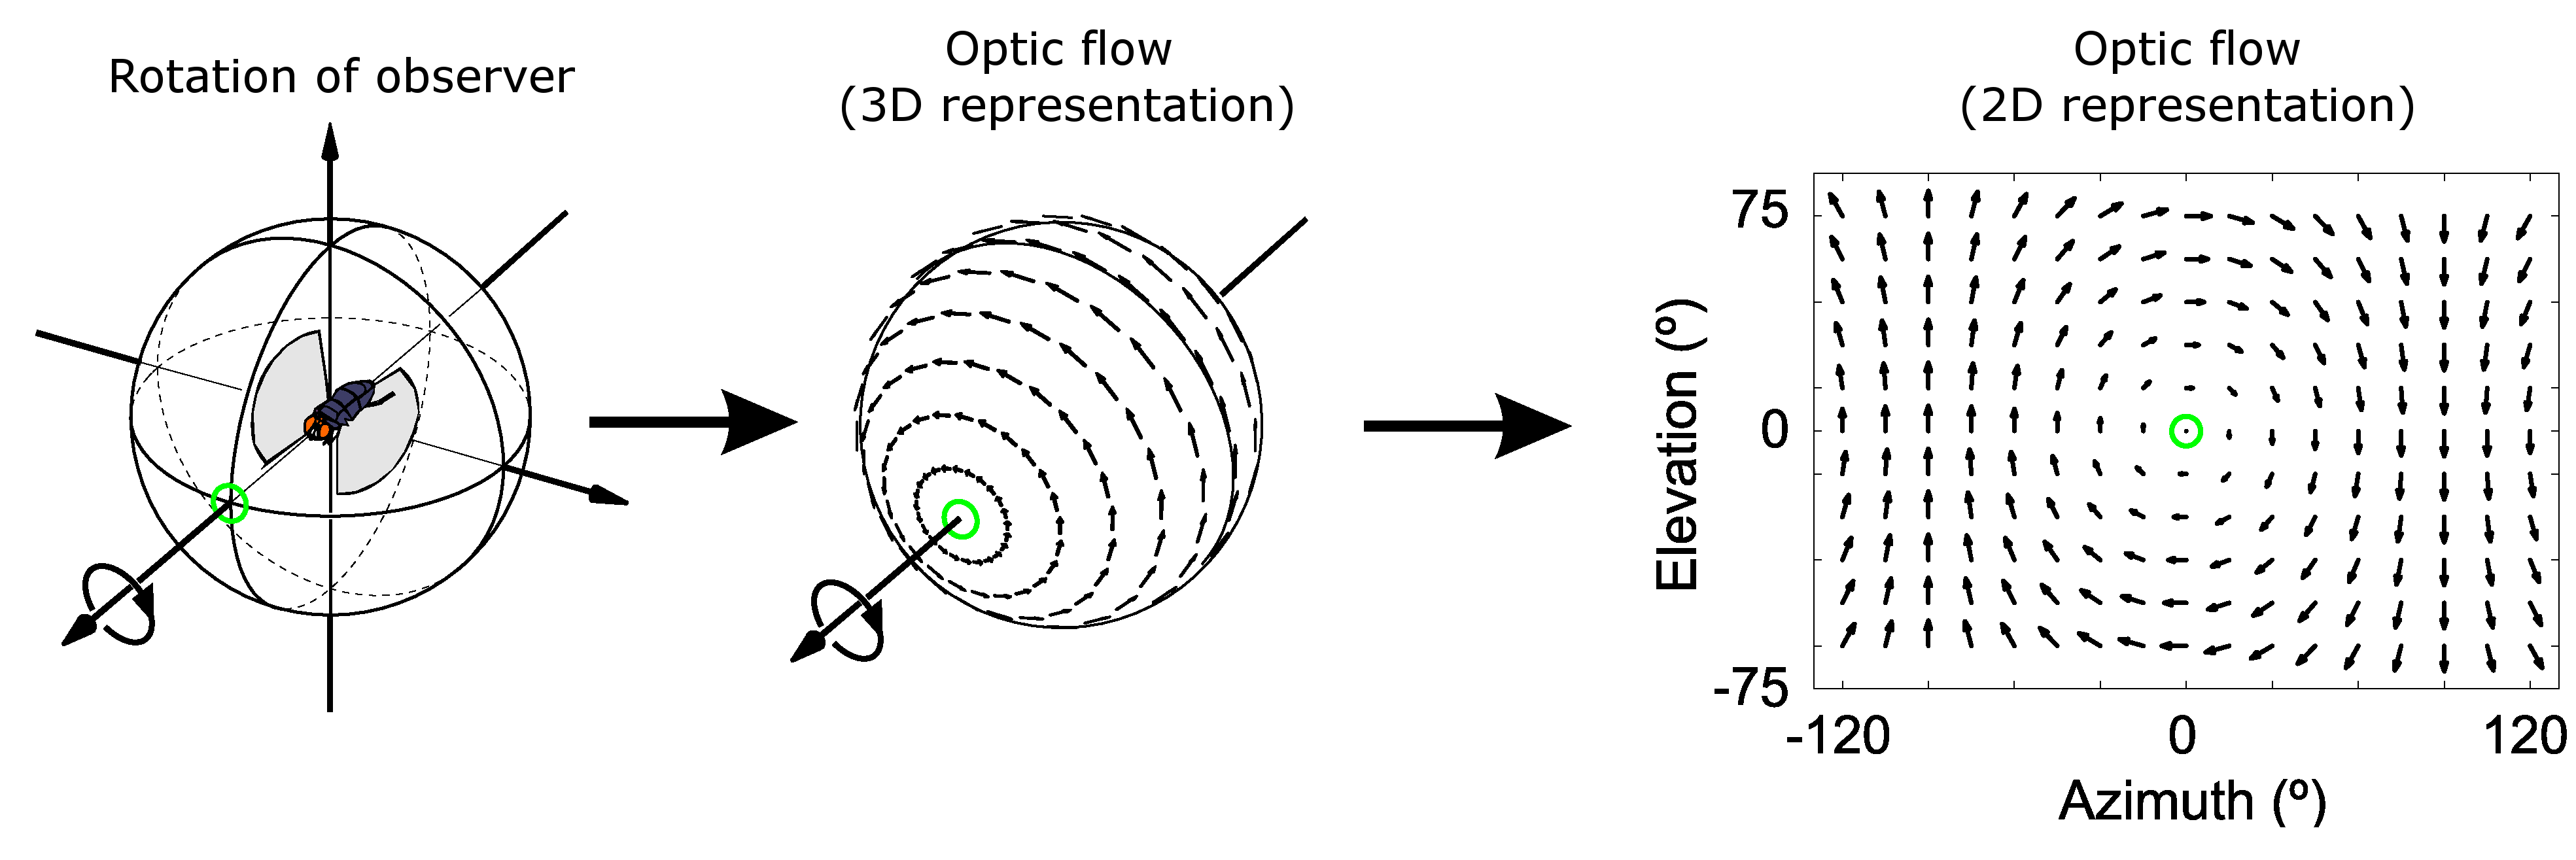
\includegraphics[width=\textwidth]{Opticfloweg}
  \caption{Optical flow caused by a rotating observer~\cite{huston2008visuomotor}}
  \label{fig:opticalflow}
\end{figure}

In section \ref{sec:theory}, \nameref{sec:theory}, I will explain the assumptions behind the theoretical development and the application of the theory. Section \ref{sec:apparatus}, \nameref{sec:apparatus}, describes the tools used in the running of the experiments and discusses the experimental accuracy. Section \ref{sec:results}, \nameref{sec:results}, presents the results obtained from the various different experiments and analyses the raw data. Finally,  section \ref{sec:conclusions}, \nameref{sec:conclusions}, highlights the main results and outlines avenues for further work and development.
\chapter{Theory and design of experiment}
\label{sec:theory}

\ifpdf
    \graphicspath{{Section2/Figs/Raster/}{Section2/Figs/PDF/}{Section2/Figs/}}
\else
    \graphicspath{{Section2/Figs/Vector/}{Section2/Figs/}}
\fi

\section{Optical Flow}

Optical flow methods attempt to calculate the motion between two images, or video frames, taken at time $t$ and $t + \Delta t$ for every pixel in the images. For a 2D case a pixel at location $(x, y, t)$ with intensity $I(x, y, t)$ will have moved by $\Delta x, \Delta y$ and $\Delta t$ between the two image frames and therefore we can impose the constraint on the intensity:

\begin{align*}
  I(x, y, t) = I(\Delta x, \Delta y, \Delta t)
\end{align*}

If we assume that the movement is small, we can perform a Taylor series expansion on the constraint:

\begin{align*}
  I(\Delta x, \Delta y, \Delta t) = I(x, y, t) + \frac{\partial I}{\partial x}\Delta x+\frac{\partial I}{\partial y}\Delta y+\frac{\partial I}{\partial t}\Delta t + \dots
\end{align*}

Ignoring higher order terms, and rearranging, it follows that

\begin{align*}
  \frac{\partial I}{\partial x}\Delta x+\frac{\partial I}{\partial y}\Delta y+\frac{\partial I}{\partial t}\Delta t = 0
\end{align*}

and dividing through by $\Delta t$ we obtain

\begin{align*}
  \frac{\partial I}{\partial x}\frac{\Delta x}{\Delta t}+\frac{\partial I}{\partial y}\frac{\Delta y}{\Delta t}+\frac{\partial I}{\partial t}\frac{\Delta t}{\Delta t} = 0
\end{align*}

which simplifies to

\begin{align*}
  \frac{\partial I}{\partial x}V_x+\frac{\partial I}{\partial y}V_y+\frac{\partial I}{\partial t} = 0
\end{align*}

where $V_x,V_y$ are the $x$ and $y$ components of the velocity or optical flow of $I(x,y,t)$ and $\tfrac{\partial I}{\partial x}$, $\tfrac{\partial I}{\partial y}$ and $\tfrac{\partial I}{\partial t}$ are the derivatives of the image at $(x,y,t)$ in the corresponding directions. We can rearrange this to

\begin{align*}
  I_xV_x+I_yV_y=-I_t
\end{align*}

where $I_x$, $I_y$ and $I_t$ are $\tfrac{\partial I}{\partial x}$, $\tfrac{\partial I}{\partial y}$ and $\tfrac{\partial I}{\partial t}$ respectively. This is an equation in two unknowns, $I$ and $V$, and therefore we cannot solve it in its current form. We require additional equations which introduce an additional constraint. All optical flow methods introduce an additional constrain to enable estimation of the optical flow.

\subsection{Lucas-Kanade}

\begin{figure}[h]
  \centering
  \begin{tikzpicture}
  \draw[->] (-0.2,0) -- (4.2,0) node[right] {$x$};
  \draw[->] (0,-1.2) -- (0,2) node[above] {$f(x)$};
  \draw[color=blue,domain=0:3] plot (\x,{sin((\x) r)}) node[right] {$f(x)$};
  \draw[color=red,domain=1:4] plot (\x,{sin((\x-1) r)}) node[right] {$g(x)$};
  \end{tikzpicture}
  \caption{The 1-D case}
  \label{fig:lucas-kanade}
\end{figure}

The Lucas-Kanade~\cite{lucas-kanade} method is a well established, sparse optical flow method. In the one dimensional case, illustrated in Figure~\ref{fig:lucas-kanade}, it can be thought of as finding the horizontal displacement, $\delta$, between the curves $F(x)$ and $G(x)=F(x+\delta)$. If we assume that $\delta$ is small and that $F(x)$ is approximately linear in the area of $x$ then we can say:

\begin{align*}
F'(x) &\approx \frac{F(x+\delta)-F(x)}{\delta} \\
\therefore F(x + \delta) &\approx F(x) + \delta F'(x) 
\end{align*}

Therefore, to find the $\delta$ which minimises the $L_2$ norm we measure the difference between the curves as

\begin{align*}
E = \sum_{x}\left[F(x + \delta) - G(x)\right]^2
\end{align*}

and then to minimise the error with respect to $\delta$, we set

\begin{align*}
  0 &= \frac{\partial E}{\partial \delta} \\
  &\approx \frac{\partial}{\partial \delta}\sum_{x}\left[F(x) + \delta F'(x) - G(x)\right]^2 \\
  &= \sum_{x}2F'(x)\left[F(x) + \delta F'(x) - G(x)\right]
\end{align*}

from which

\begin{align*}
  \delta \approx \frac{\sum_{x}F'(x)\left[G(x) - F(x)\right]}{\sum_{x}F'(x)^2}
\end{align*}

We can generalise this to n-dimensions as follows. We still wish to minimise the $L_2$ norm as a measure of error

\begin{align*}
  E = \sum_{x \in \mathbb{R}}\left[F(x + \delta) - G(x)\right]^2
\end{align*}

where x and $\delta$ are n-dimensional row vectors. We make a linear approximation as before

\begin{align*}
  F(x + \delta) \approx F(x) + \delta\frac{\partial}{\partial x}F(x)
\end{align*}

Where

\begin{align*}
  \frac{\partial}{\partial x} = \left[\frac{\partial}{\partial x_1} \frac{\partial}{\partial x_2} \dots \frac{\partial}{\partial x_n}\right]^T
\end{align*}

and as before to minimise the error with respect to $\delta$, we set

\begin{align*}
0 &= \frac{\partial E}{\partial \delta} \\
&\approx \frac{\partial}{\partial \delta}\sum_{x}\left[F(x) + \delta \frac{\partial F}{\partial x} - G(x)\right]^2 \\
&= \sum_{x}2\frac{\partial F}{\partial x}\left[F(x) + \delta \frac{\partial F}{\partial x} - G(x)\right]
\end{align*}

from which

\begin{align*}
  \delta = \left[\sum_{x}\left(\frac{\partial F}{\partial x}\right)^T\left[G(x) - F(x)\right]\right]\left[\sum_{x}\left(\frac{\partial F}{\partial x}\right)^T\left(\frac{\partial F}{\partial x}\right)\right]^{-1}
\end{align*}

\subsection{Farnebäck}

Farnebäck optical flow~\citep{farneback} is classified as a dense optical flow method. Using this method each neighbourhood of pixels is approximated by a quadratic polynomial of the form:

\begin{align*}
f(x) \approx x^TAx+b^tx+c
\end{align*}

In the one dimensional case is shown in figure~\ref{fig:farneback}.

\begin{figure}[h]
  \centering
  \begin{tikzpicture}
  \draw[->] (-0.2,0) -- (4.2,0) node[right] {$x$};
  \draw[->] (0,-1.2) -- (0,2) node[above] {$f(x)$};
  \draw[color=blue,domain=0:3] plot (\x,{sin((\x) r)}) node[right] {$f(x)$};
  \draw [->] (.5,0) -- (.5,.5); 
  \draw [->] (1,0) -- (1,.85); 
  \draw [->] (1.5,0) -- (1.5,1); 
  \draw [->] (2,0) -- (2,.9);
  \draw [->] (2.5,0) -- (2.5,.6); 
  \end{tikzpicture}
  \caption{The 1-D case}
  \label{fig:farneback}
\end{figure}

For the general case, if we consider the polynomial $f_1(x) \approx x^TA_1x+b_1^Tx+c_1$ which is shifted by a displacement $\delta$

\begin{align*}
f_2(x) &= f_1(x-\delta) \\
&= (x-\delta)^T A_1 (x-\delta) + b_1^T (x-\delta) + c_1 \\
&= x^TA_1x + (b_1 - 2A_1\delta)^Tx + \delta^TA_1\delta -b_1^T\delta + c_1 \\
&\equiv x^TA_2x + b_2^Tx + c_2
\end{align*}

We can therefore equate the coefficients of $f_1(x)$ and $f_2(x)$ which yields

\begin{align*}
A_2 &= A_1 \\
b_2 &= b_1 - 2A_1\delta \\
c_2 &= \delta^TA_1\delta - b_1^T\delta + c_1
\end{align*}

Thus if $A_1$ is non-singular we can solve for the translation $\delta$

\begin{align*}
b_2 &= b_1 - 2A_1\delta \\
2A_1\delta &= -(b_2-b_1) \\
\delta &= -\frac{1}{2}A_1^{-1}(b_2-b_1)
\end{align*}

\subsection{SimpleFlow}

SimpleFlow is a combination of both dense and sparse optical flow, it only runs a full flow estimation at a few key pixels, and linearly interpolates the rest of the flow, thus it is classified as \textit{semi-dense} optical flow~\citep{simpleflow}. At the key pixels a likelihood model is used, that is, we seek flow vectors $(u,v)$ such that $F_t(x,y)$ and $F_{t+1}(x+u,y+v)$ are similar. This is modelled by the energy term:

\begin{align*}
e(x,y,u,v) = {\lVert F_t(x,y)+F_{t+1}(x+u,y+v)\rVert}^2 
\end{align*}

that corresponds to the likelihood probability $p \propto \exp(-e)$~\citep{rosenberg1997representing}


SimpleFlow assumes that the flow is locally smooth, however it does not rely on a simple pairwise term such as $\left|\left|(u_1,v_1)-(u_2,v_2)\right|\right|^2$ as is often used as pairwise terms link flow estimates at several pixels therefore making optimization problem harder to solve. Instead SimpleFlow requires the flow vector $(u_0,v_0)$ at pixel $(x_0, y_0)$ to not only be a good estimate for the optical flow of $(x_0, y_0)$, but at other pixels in the local neighbourhood, $\mathcal{N}_0$. This can be expressed as

\begin{align*}
  (u_0,v_0) = \arg\min_{(u,v)\in\Omega}\prod_{(x,y)\in\mathcal{N}_0}p(x,y,u,v)
\end{align*}

where $\Omega$ is the set of all possible $(u,v)$ vectors considered. This produces a smoother estimate of the optical flow of $(x, y)$. We can better understand this behaviour in the negative log-likelihood (or energy cost) domain where we try to find the lowest cost flow vector for the pixel $(x_0,y_0)$

\begin{align*}
  (u_0,v_0) = \arg\min_{(u,v)\in\Omega} \sum_{(x,y)\in\mathcal{N}_0} e(x,y,u,v)
\end{align*}

The smoothness prior amounts to smoothing the  the likelihood term instead of adding a pairwise term. As a consequence, finding a minimizer remains simple since there is no interaction between the unknowns, the solution at a pixel does not depend on the solution at its neighbours.

Smoothing with a box filter would not differentiate between pixels within $\mathcal{N}_0$, e.g. it would ignore edges. Therefore weights must be added to account for how pixels relate to each other. Two weighting functions are required, $w_d$ for the distance between pixels and $w_c$ for the colour difference. This is represented as:

\begin{align*}
  E(x_0, y_0, u, v) &= \sum_{(x, y) \in \mathcal{N}_0} w_d w_c e(x, y, u, v) \\
  \text{with } w_d &= \exp\left(-\left|\left| (x_0, y_0) - (x, y)\right|\right|^2 / 2\sigma_d\right) \\
  \text{and } w_c &= \exp\left(-\left|\left| F_t(x_0, y_0) - F_t(x, y)\right|\right|^2 / 2\sigma_c\right)
\end{align*}
\chapter{Apparatus and experimental techniques}
\label{sec:apparatus}

\ifpdf
    \graphicspath{{Section3/Figs/Raster/}{Section3/Figs/PDF/}{Section3/Figs/}}
\else
    \graphicspath{{Section3/Figs/Vector/}{Section3/Figs/}}
\fi

\section{OpenCV}

To aid in implementing image processing algorithms, including optical flow methods, OpenCV~\cite{opencv} was used. OpenCV (Open Source Computer Vision Library) is an open source computer vision and machine learning software library. A precompiled binary does not exist for the Raspberry Pi, so it was necessary to compile it from source and write instructions on how to do so. On the Raspberry Pi the compilation time is around 10-12 hours depending on the overclock used. 

Also included in code listing~\ref{lst:opencv}, Appendix~\ref{sec:appendix} are instructions on how to allow the Raspberry Pi camera to interface with the operating system. An extra driver (UV4l-raspi~\cite{uv4l}) is required, however a precompiled binary is available in this case. Also included in written up instructions on how to install SimpleCV~\cite{simplecv}, a Python wrapper for OpenCV. SimpleCV was not used in the following experiments due to the performance benefits of C/C++ over Python, however the instructions are included as they will be provided on the OpenLabTools website.

In order to use the library to perform a comparison, an object oriented program which contained implementations of the Lucas-Kanade, Farnebäck, and SimpleFlow algorithms. The program was designed to be run from the command line, so that it's operation can be scripted using BASH or any other scripting language, and also so as not to waste unnecessary resources on drawing a GUI. The full code listing for the program can be seen online~\cite{github}. Listed below is the help message for the \verb|optical-flow| program. Note that multiple optical flow algorithms can be applied to the same input file at once i.e. \verb|./optical-flow -fls -o output.avi input.avi| will run Lucas-Kanade, Farnebäck and SimpleFlow optical flow algorithms on the file \verb|input.avi| and will output \verb|output.lucas-kanade.avi, output.farneback.avi| and \verb|output.simpleflow.avi|
 
\singlespacing
\begin{verbatim}
  Usage: ./optical-flow [options] file...
  Options:
    -h, --help          Display this help message
    -v, --version       Display the program version
    -o, --output        The file you wish to write to
    -f, --farneback     Use the Farneback optical flow method
    -l, --lucas-kanade  Use the Lucas-Kanade optical flow method
    -s, --simpleflow    Use the Simpleflow optical flow method
\end{verbatim}
\onehalfspacing

\section{Comparison}

The first area investigated was a comparison between the three optical flow algorithms previously listed for speed and accuracy on the Raspberry Pi. Each algorithm will be tested using an artificial dataset, and a real world dataset. Accuracy is only able to be measured quantitatively for the artificial dataset, and it is measured by taking the $L_2$ norm of the optical flow output from each algorithm and comparing it to the optical flow calculated. This technique is explained further in the section beneath. The speed of each algorithm is measured for both the artificial dataset and the real world dataset, and it is measured by calculating the mean processing time per pair of video frames processed. 

Timing data was output from the \verb|optical-flow| program to stdout, however when the comparison process was automated, this was redirected to a text file. A typical output can be seen beneath

\singlespacing
\begin{verbatim}
Output file fracture.lucas-kanade.avi using Lucas-Kanade optical flow

Frame 1 took 0.24s to process
...
Frame 11 took 75.38s to process

Processing complete for fracture.lucas-kanade.avi
\end{verbatim}
\onehalfspacing

In order to process the large amount of timing information in an accurate and repeatable manner, a python script was authored. The full script can be seen in code listing~\ref{lst:timings} of Appendix~\ref{sec:appendix}. A typical output from the script can be seen beneath

\singlespacing
\begin{verbatim}
Output file fracture.lucas-kanade.avi using Lucas-Kanade optical flow
74.60s average per frame
\end{verbatim}
\onehalfspacing

In order to process the large amount of optical flow information, and compare it to the known vector flow field, the output from \verb|optical-flow| first has to be converted into a form that can be read by MATLAB. \verb|optical-flow| outputs vector field information in the YAML (Yet Another Markup Language) format, with Farnebäck and SimpleFlow directly outputting the vector field, whereas Lucas-Kanade outputs two arrays, \verb|prevPts| and \verb|nextPts|, which hold the coordinate pairs of the pixels being tracked in frame $F_t$ and followed by their position in frame $F_{t+1}$. An example of the vector field data output from the Farnebäck algorithm is listed below

\singlespacing
\begin{verbatim}
%YAML:1.0
FlowField : !!opencv-matrix
rows: 240
cols: 240
dt: "2f"
data: [ 0., 0., 0., 0., 0., 0., 0., 0., 0., 0., 0., 0., 0., 0., 0.,
...
       -4.66855984e-34, -1.97913447e-33, -3.70633920e-34 ]
\end{verbatim}
\onehalfspacing

Therefore a Python script was authored in order to convert this output into something which could be more easily processed. The full script can be seen in code listing~\ref{lst:process} of Appendix~\ref{sec:appendix}. 

\subsection{Artificial Data}

The artificial dataset consists of the MATLAB \verb|checkerboard| pattern, which has five different affine transformations repeatedly applied to it in order to generate five different artificial data sequences. The sequences include: translation, rotation, scaling, shearing and fracture. Frames from each of the sample sequences can be seen in Figure~\ref{fig:artificial} below.

\begin{figure}[h]
  \centering
  \begin{subfigure}[b]{.16\textwidth}
    
\includegraphics[width=\textwidth]{orig}
    \caption{Original}
    \label{fig:orig}
  \end{subfigure}
  \begin{subfigure}[b]{.16\textwidth}
    
\includegraphics[width=\textwidth]{translate}
    \caption{Translate}
    \label{fig:trans}
  \end{subfigure}
  \begin{subfigure}[b]{.16\textwidth}
    
\includegraphics[width=\textwidth]{rotate}
    \caption{Rotate}
    \label{fig:rot}
  \end{subfigure}
  \begin{subfigure}[b]{.16\textwidth}
    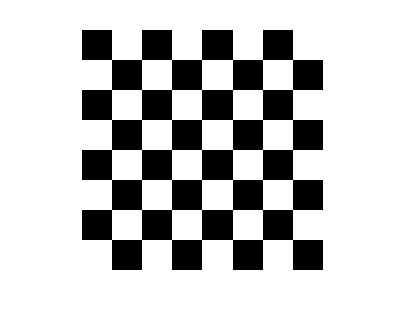
\includegraphics[width=\textwidth]{scale}
    \caption{Scale}
    \label{fig:scale}
  \end{subfigure}
  \begin{subfigure}[b]{.16\textwidth}
    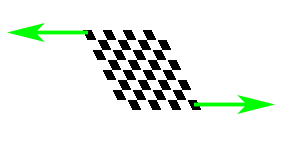
\includegraphics[width=\textwidth]{skew}
    \caption{Shear}
    \label{fig:skew}
  \end{subfigure}
  \begin{subfigure}[b]{.16\textwidth}
    
\includegraphics[width=\textwidth]{disjoint}
    \caption{Fracture}
    \label{fig:disj}
  \end{subfigure}
  \caption{Artificial dataset}
  \label{fig:artificial}
\end{figure}

Each of the above sequences was generated by the following affine transformation matrices respectively:

\begin{align*}
  \begin{bmatrix}
  1 & 0 & T_x \\
  0 & 1 & T_y \\
  0 & 0 & 1 \\
  \end{bmatrix}
  \hspace{1em}
  \begin{bmatrix}
  \cos(\theta) & -\sin(\theta) & 0 \\
  \sin(\theta) & \cos(\theta) & 0 \\
  0 & 0 & 1 \\
  \end{bmatrix}
  \hspace{1em}
  \begin{bmatrix}
  S_x & 0 & 0 \\
  0 & S_y & 0 \\
  0 & 0 & 1 \\
  \end{bmatrix}
  \hspace{1em}
  \begin{bmatrix}
  1 & 0 & 0 \\
  S & 1 & 0 \\
  0 & 0 & 1 \\
  \end{bmatrix}
\end{align*}

From left to right, the above transformation matrices represent: a translation, of $T_x$ pixels in the x-direction and $T_y$ pixels in the y direction; a rotation of $\theta$ degrees about the centroid of the \verb|checkerboard| pattern; a scaling of $S_x$ in the x-direction and $S_y$ in the y direction; A shear parallel to the x-axis of S pixels i.e. $x' = x + ky$. The fracture is represented in MATLAB as two separate translations applied to two halves of the original \verb|checkerboard| pattern. For this dataset $T_x = -5i, T_y = -5i, \theta = 1^\circ, S_y = (i+1)/2, S_x = (i+1)/2$ and $S = .5$ where $i$ is the frame of the video being generated. The fracture had transformation equivalent to a translation with $T_y = sgn(y)2i$ applied to it, where the centroid of the \verb|checkerboard| pattern is coincident with the origin. Each transformation is applied repeatedly in order to generate sample sequences ten frames long. The MATLAB code used to generate the rotation sample sequence can be seen in code listing~\ref{lst:rotation}. The complete MATLAB code listing used to generate all the sample sequences can be seen in code listing~\ref{lst:generate} in Appendix~\ref{sec:appendix}.

\singlespacing
\begin{lstlisting}[language=MATLAB,caption={MATLAB code for creating rotation sample sequence},label=lst:rotation]
  theta=1;
  tform=affine2d([cosd(theta) -sind(theta) 0; sind(theta) cosd(theta) 0; 0 0 1]);
  writerObj = VideoWriter('rotate.avi');
  open(writerObj);
  frame=uint8(padarray(orig,[200 200],255).*255);
  writeVideo(writerObj,frame);
  r=imwarp(orig,tform,'FillValue',255);
  for i=1:10
    dr=size(r,1)-size(orig,1);
    dc=size(r,2)-size(orig,2);
    frame=uint8(padarray(r,[200-dr/2 200-dc/2],255).*255);
    writeVideo(writerObj,frame);
    r=imwarp(r,tform,'FillValue',255);
  end
  close(writerObj);
\end{lstlisting}
\onehalfspacing

In order to evaluate the algorithms more rigorously, the five sample sequences were sub sampled by $\frac{1}{2}, \frac{1}{4}, \frac{1}{8}$ and $\frac{1}{16}$ of the original size. In addition, as the Lucas-Kanade algorithm is a sparse optical flow algorithm, in order to make the comparison more rigorous when selecting points to track a set of all the pixels in the image was passed to the algorithm. This effectively makes the Lucas-Kanade algorithm a dense optical flow algorithm.

In order to measure the accuracy of the optical flow algorithm, as stated previously, it is required to know the optical flow that each of the transformations cause in the sample sequences. Therefore it was necessary to calculate the velocity field of each of the transformations as they were applied to the \verb|checkerboard| pattern. The MATLAB code written to calculate the velocity field for an arbitrary image which has an arbitrary transformation matrix applied to it can be seen in full in code listing~\ref{lst:velflow} in Appendix~\ref{sec:appendix}, however the key parts of the algorithm can be seen below, in code listing~\ref{lst:velfield}.

\singlespacing
\begin{lstlisting}[language=MATLAB,caption={MATLAB code to calculate the velocity field of a transformation matrix},label=lst:velfield]
% Set up matrix of points r0.
r0 = ones(n*m, 3);
n_ = -n/2;
m_ = -m/2;
for i = 1:n
  r0(i:m:(n*m),2) = n_;
  n_ = n_ + 1;
end
for j = 1:m
  r0((n*(j-1) + 1):n*j,1) = m_;
  m_ = m_ + 1;
end

% Calculate new positions for all points r0 after transformation under
%   tform, which are r1.
r1 = r0*tform.T;
r1(:,1) = r1(:,1)./r1(:,3);
r1(:,2) = r1(:,2)./r1(:,3);

% Eliminate third column (now unneeded)
r0_ = r0(:,1:2);
r1_ = r1(:,1:2);

% Calculate stacked matrix of velocities, v.
v = r1_ - r0_;

% Reshape v into V
V = reshape(v, [n m 2]);
r0 = reshape(r0_, [n m 2]);
r1 = reshape(r1_, [n m 2]);
\end{lstlisting}
\onehalfspacing

It should be noted that while we are only investigating individual affine transformations, the code listed in code listing~\ref{lst:velfield} and the full code in code listing~\ref{lst:velflow} in Appendix~\ref{sec:appendix} also work for arbitrary affine transformation matrices, in addition to projective transformation matrices.

Figure~\ref{fig:shearfield} shows the output from the velocity field calculation plotted using the MATLAB \verb|quiver| function. While at this scale is is impossible to discern the magnitude, or the direction to any degree of accuracy, it can be seen that the magnitude of the velocity grows in proportion to the absolute value of the y-coordinate. 

\begin{figure}[h]
  \centering
  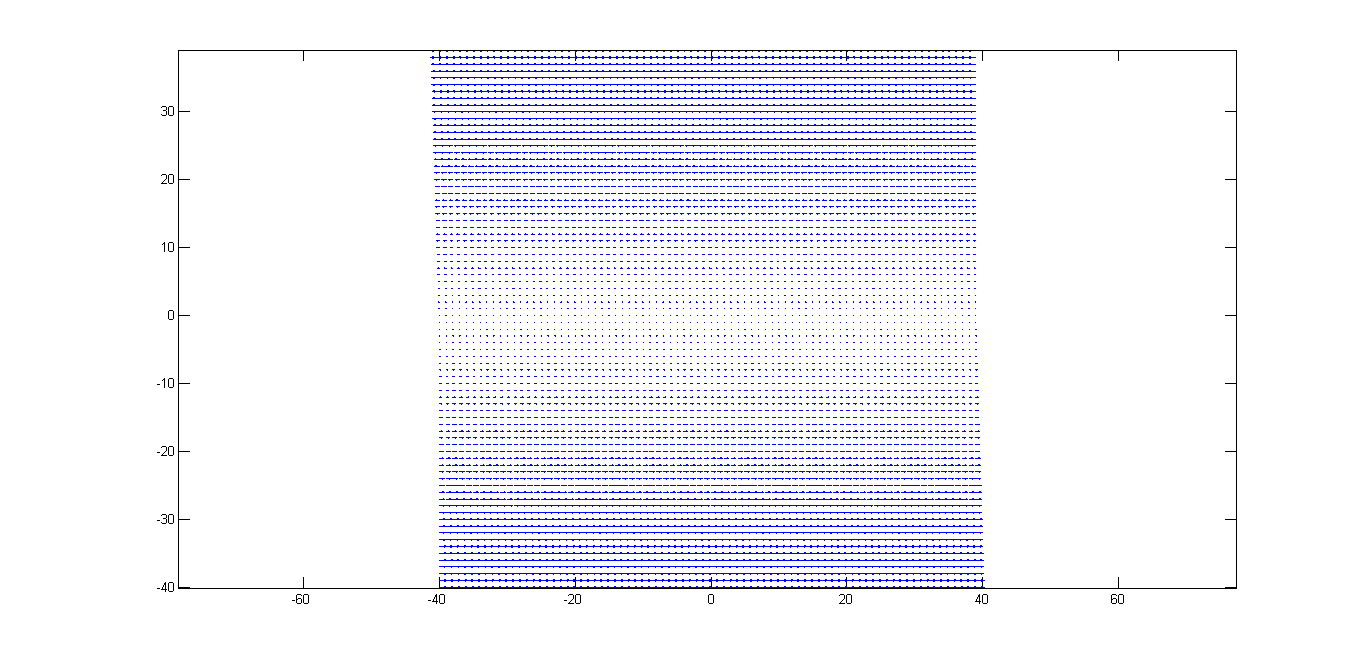
\includegraphics[width=\textwidth]{shear.png}
  \caption{Velocity field calculate for a shear}
  \label{fig:shearfield}
\end{figure}

\subsection{Real World Data}

In order to examine the algorithms in a real world scenario I was graciously provided with data sets from Dr Alexandre Kabla~\cite{harris2012characterizing}, a lecturer and researcher in CUED, and Mustafa Kamal, A PhD student in the Hopkinson Lab. Figure~\ref{fig:kamal} shows flow-flame interactions and comes from a high speed PIV dataset. Figure~\ref{fig:kabla} shows a cultured cell monolayer undergoing tensile testing.

\begin{figure}[htbp!]
  \centering
  \begin{subfigure}[b]{0.49\textwidth}
    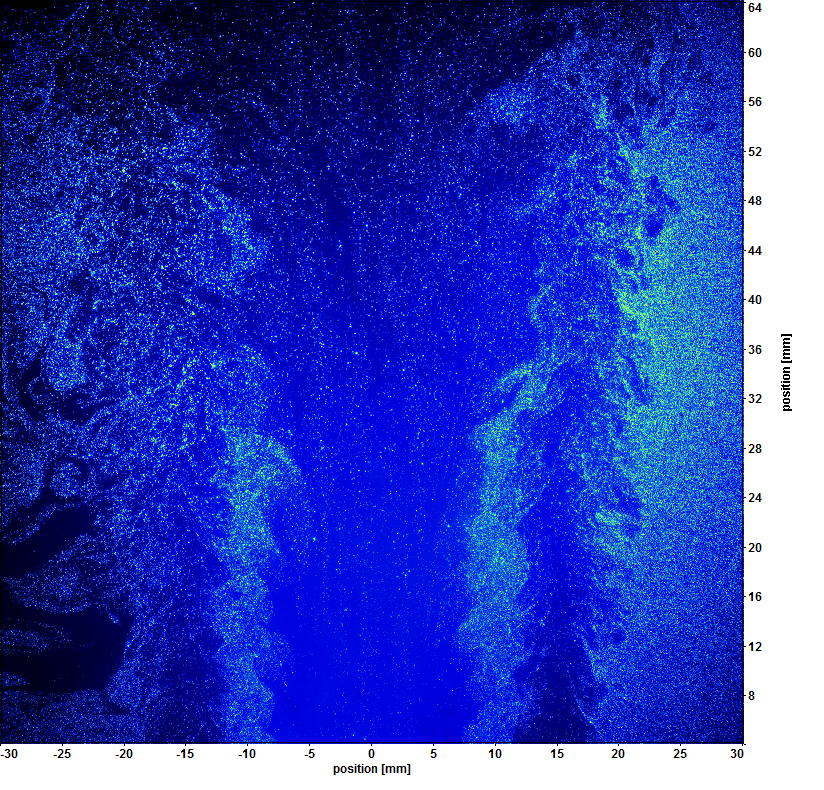
\includegraphics[width=\textwidth]{kamal}
    \caption{Provided by Mustafa Kamal}
    \label{fig:kamal}
  \end{subfigure}
  \begin{subfigure}[b]{0.49\textwidth}
    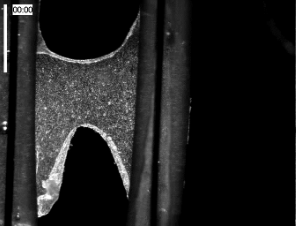
\includegraphics[width=\textwidth]{kabla}
    \caption{Provided by Dr. Alexandre Kabla}
    \label{fig:kabla}
  \end{subfigure}
  \caption{Real world data sets used}
  \label{fig:realworld}
\end{figure}

As there is no accurate, prior knowledge of the vector flow field, these datasets can only be used to compare the three optical flow algorithms for speed quantitatively, and for accuracy qualitatively. Also, for testing of real world data the Lucas-Kanade algorithm was used as a true sparse optical flow algorithm as opposed to its use in testing the artificial data where it was forced to track all pixels. It selected which pixels to track by calculating the minimal eigenvalue of gradient matrices for corner detection.
\chapter{Results and discussion}
\label{sec:results}

\ifpdf
    \graphicspath{{Section4/Figs/Raster/}{Section4/Figs/PDF/}{Section4/Figs/}}
\else
    \graphicspath{{Section4/Figs/Vector/}{Section4/Figs/}}
\fi

\section{Comparison}

\subsection{Artificial Data}

Plotted in figures~\ref{fig:rotate} to~\ref{fig:translate}, and listed in tables~\ref{tab:rotation} to~\ref{tab:fracture} of Appendix~\ref{sec:appendix3}, are the timing and error (per pixel) values measured and calculated, respectively, averaged over three runs of each optical flow algorithm, so as to eliminate non-deterministic effects, for each of the affine transformations. The video sequences used varied from 480x480 pixels for a subsampling of 1, to 30x30 pixels for a subsampling of 16. The results shown in tables~\ref{tab:rotation} to~\ref{tab:fracture} in Appendix~\ref{sec:appendix3} are rounded to two decimal places, however the plots found in figures~\ref{fig:rotate} to~\ref{fig:translate} show the true values. The author was unable to construct the space dependent flow field required to calculate the accuracy of the fracture transformation, therefore only the timing information is included in table~\ref{tab:fracture}. However, it should be noted that the fracture transformation is effectively a translation.

\begin{figure}[h]
  \centering
  \makebox[\textwidth][c]{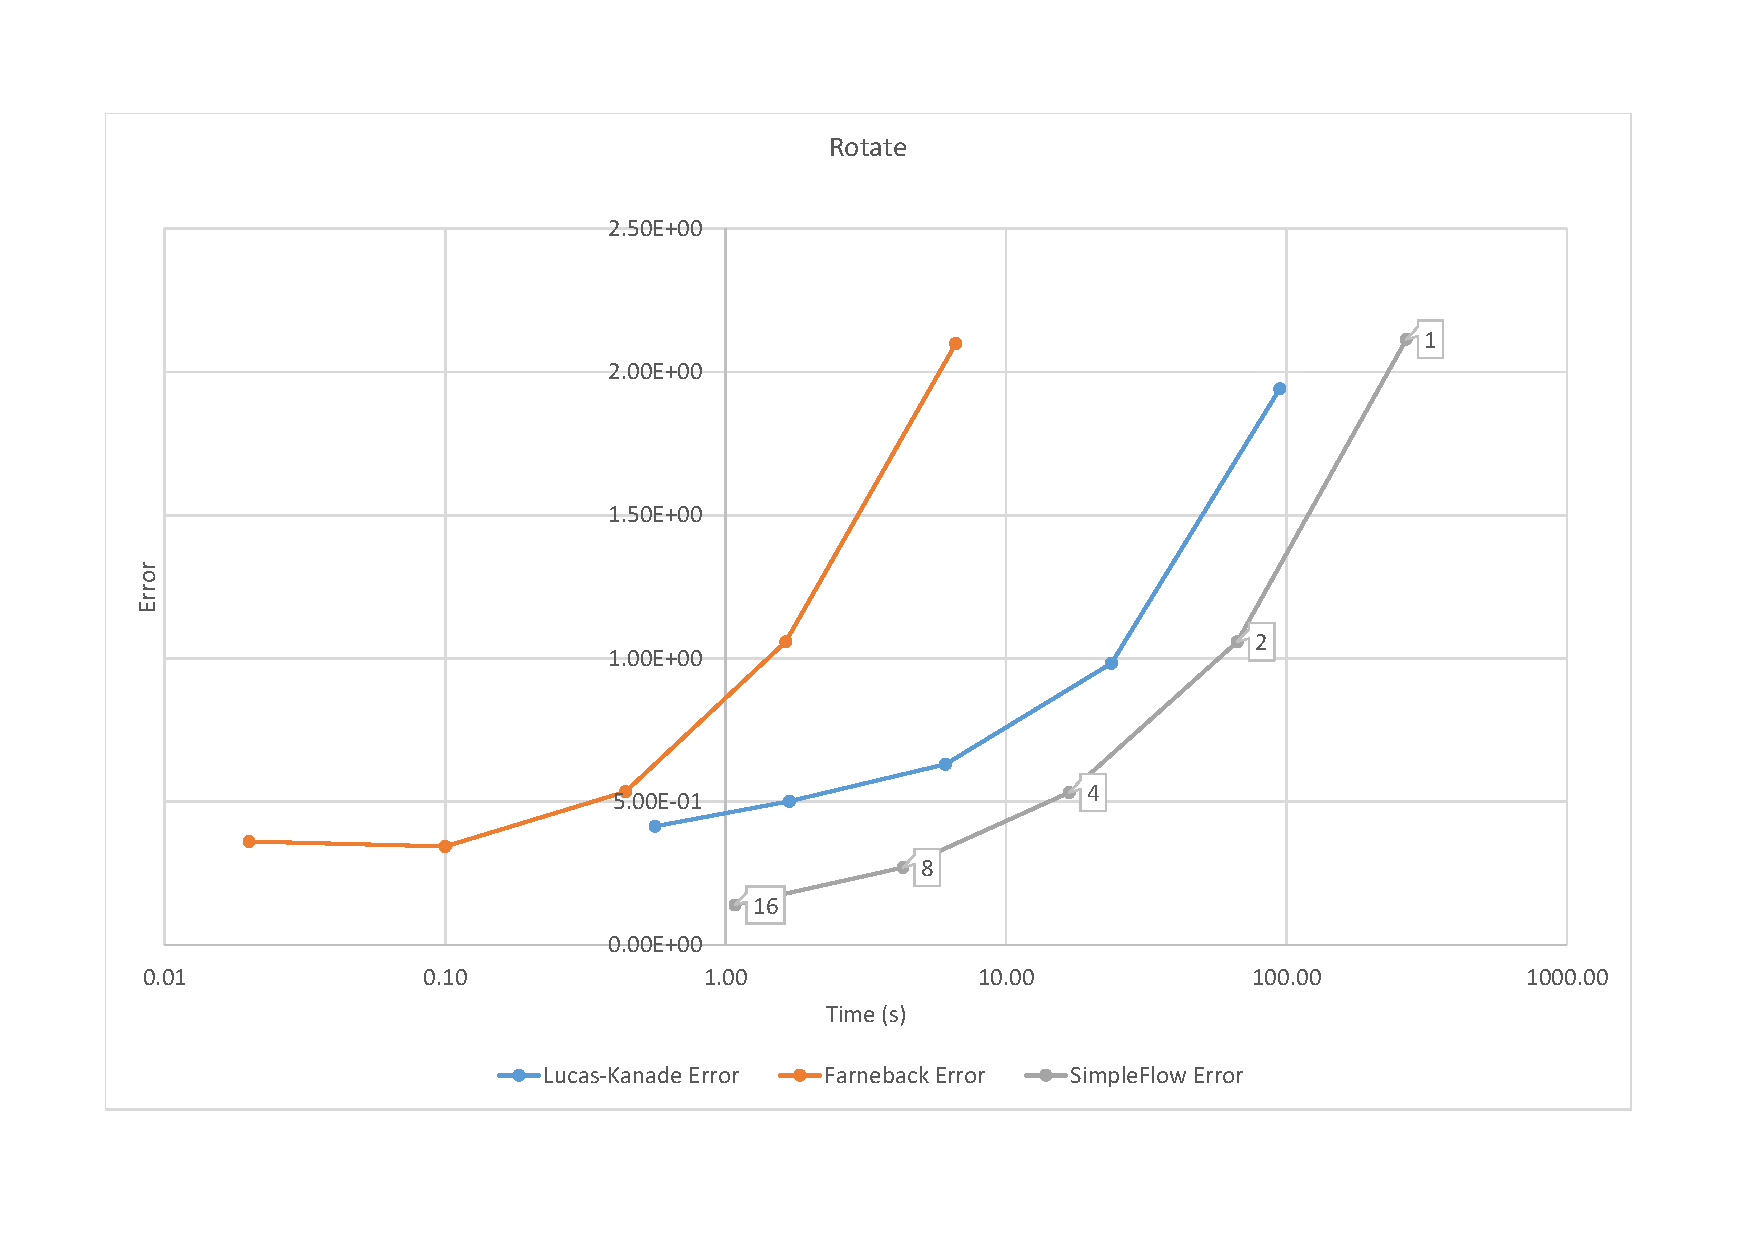
\includegraphics[width=1.2\textwidth]{rotate.pdf}}
  \caption{Rotate: Accuracy vs Speed}
  \label{fig:rotate}
\end{figure}

Firstly taking the results for the rotation transformation, plotted in figure~\ref{fig:rotate} and listed in table~\ref{tab:rotation} of Appendix~\ref{sec:appendix3}, it is plain to see that the error per pixel, and the processing time increases as the subsampling decreases, and conversely as the image size increases. For the higher subsampling in the rotation transformation the SimpleFlow algorithm has a lower error per pixel, however this is at the cost of a longer processing time per frame of video. As the sample sequences grow larger, the Farnebäck algorithm starts to show an advantage in the error per pixel. Consistently throughout the different frame sizes, the Lucas-Kanade method is the fastest.

\begin{figure}[h]
  \centering
  \makebox[\textwidth][c]{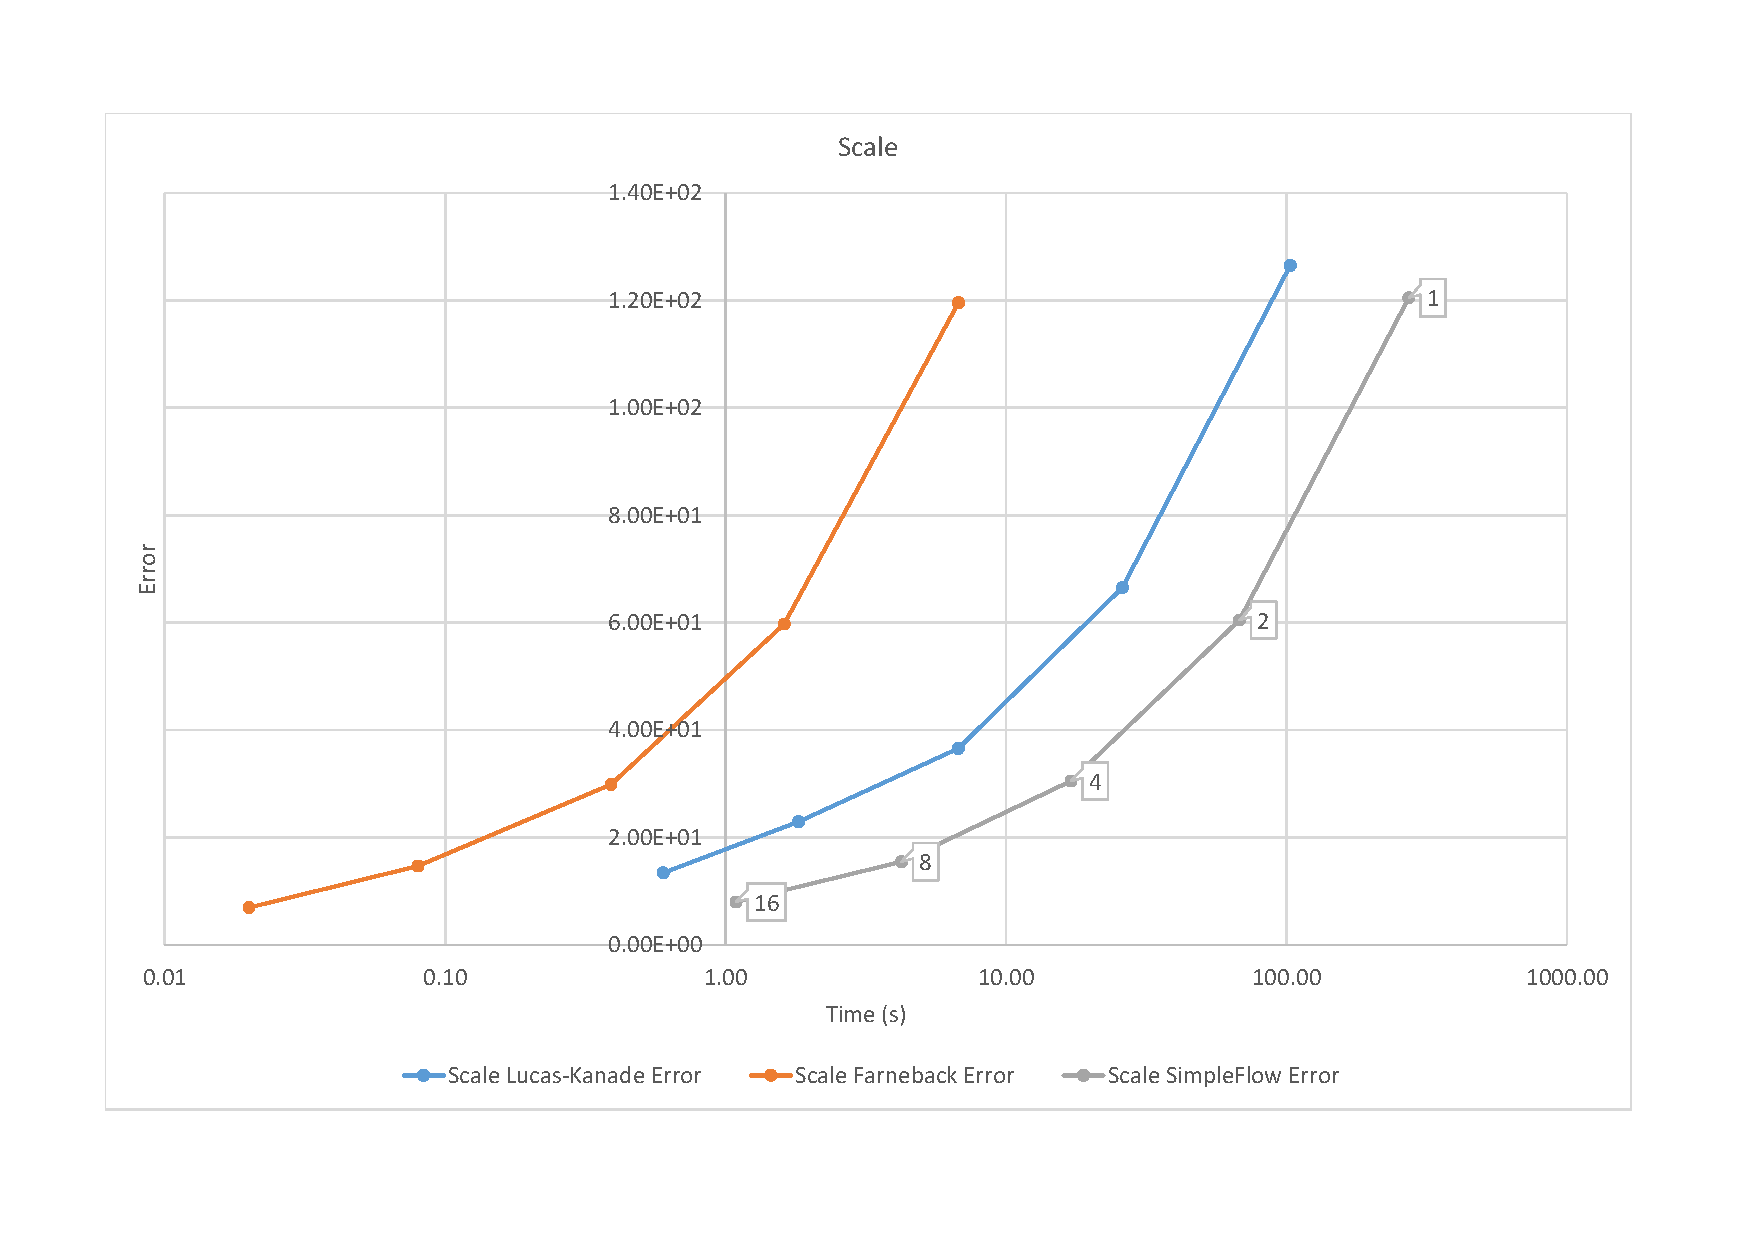
\includegraphics[width=1.2\textwidth]{scale.pdf}}
  \caption{Scale: Accuracy vs Speed}
  \label{fig:scaling}
\end{figure}

Looking at the results for the scaling transformation, plotted in figure~\ref{fig:scaling} and listed in table~\ref{tab:scale} of Appendix~\ref{sec:appendix3}, they are similar to those of the rotation transformation. That is to say, that the SimpleFlow algorithm has the longest processing time, while the Lucas-Kanade algorithm has the shortest processing time, with the Farnebäck algorithm lying somewhere in between. The main difference between scaling and rotation is that the Lucas-Kanade algorithm consistently wins out against the other two on accuracy.

\begin{figure}[h]
  \centering
  \makebox[\textwidth][c]{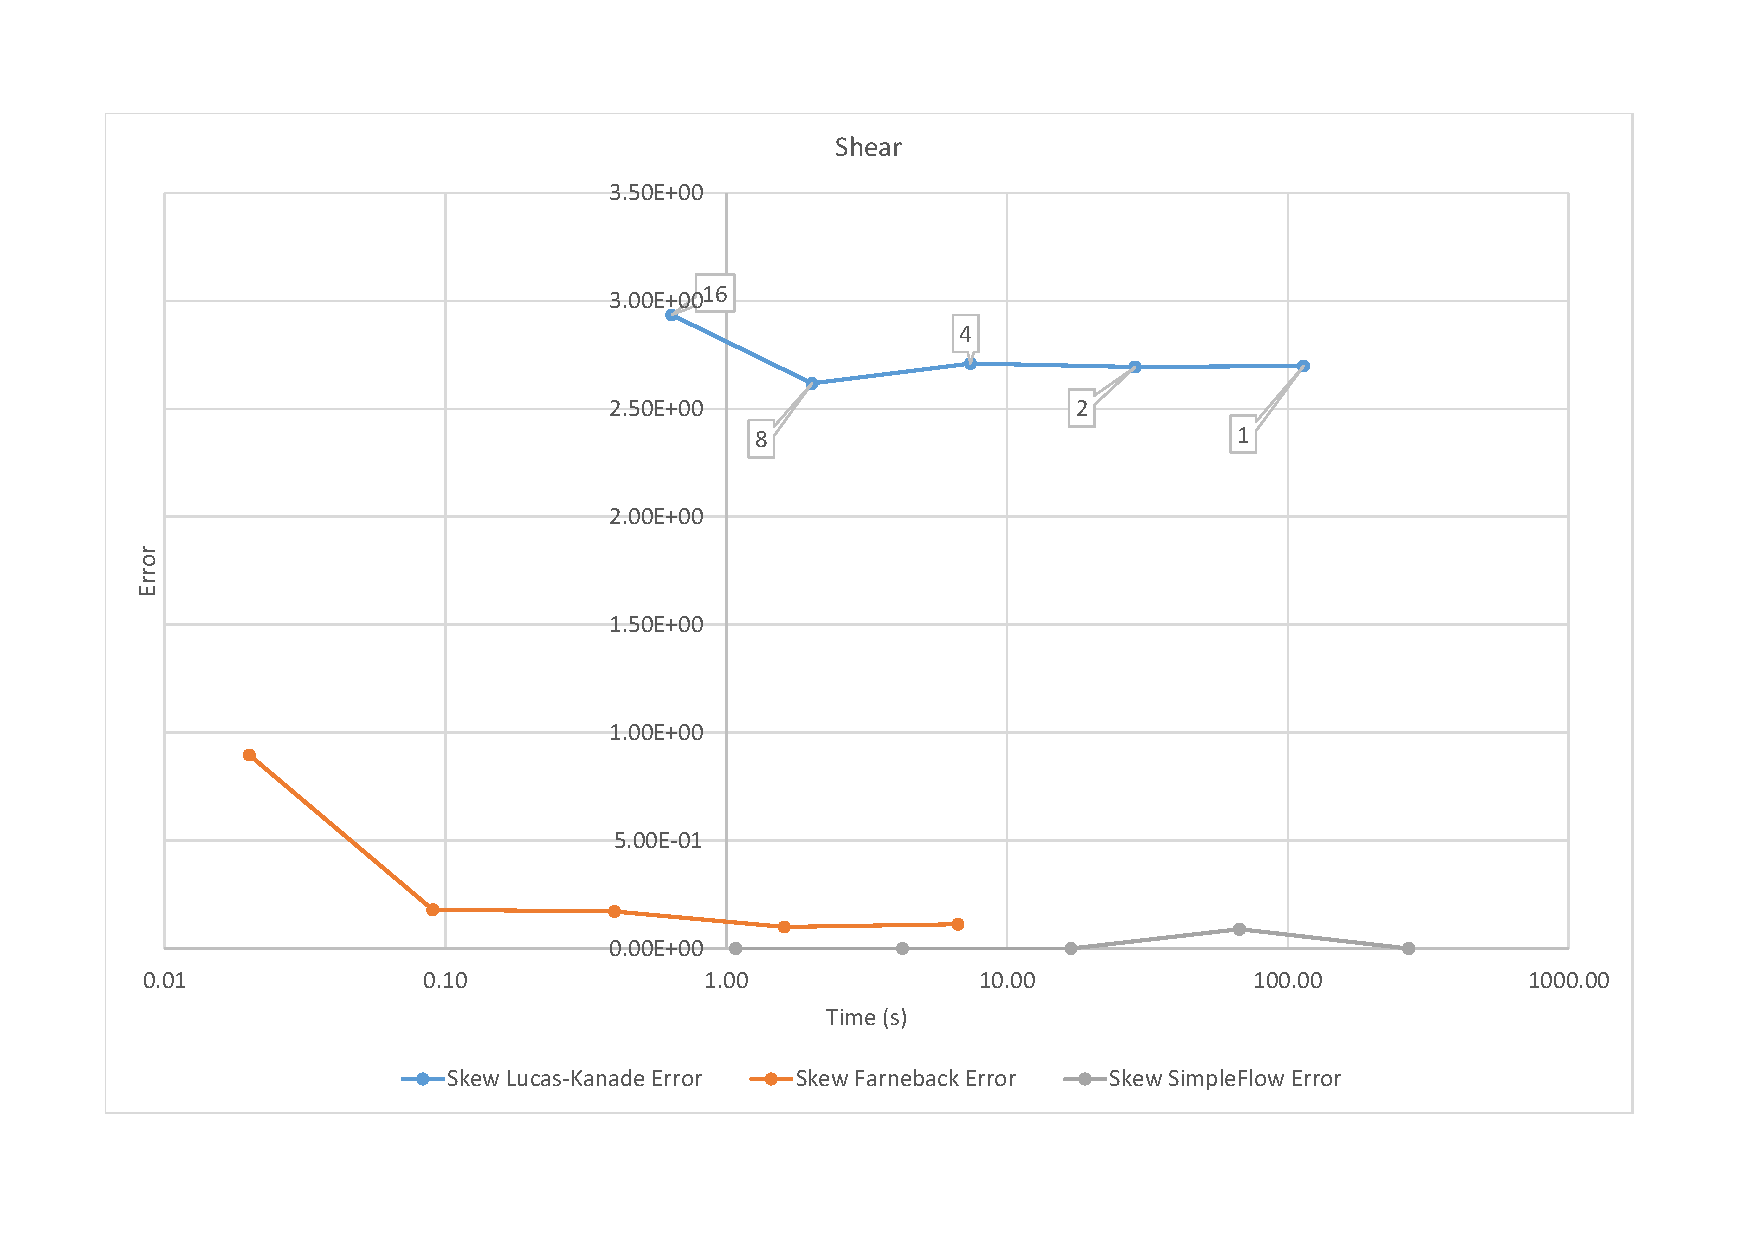
\includegraphics[width=1.2\textwidth]{shear.pdf}}
  \caption{Shear: Accuracy vs Speed}
  \label{fig:shear}
\end{figure}

Looking at the results for the shear transformation, plotted in figure~\ref{fig:shear} and listed in table~\ref{tab:shear} of Appendix~\ref{sec:appendix3}, they present a different view to either of the two transformations previously mentioned. All three algorithms have approximately uniform error across all subsampling amounts, however the processing time increases as the subsampling decreases, or conversely, as the frame size increases. SimpleFlow presents the lowest error per pixel of all three optical flow algorithms, however on larger images it has the longest processing time per frame. The other two algorithms present higher errors per pixel, however the Farnebäck algorithm appears to be very efficient at processing shear transformations compared to the other two algorithms.

\begin{figure}[h]
  \centering
  \makebox[\textwidth][c]{
\includegraphics[width=1.2\textwidth]{translate}}
  \caption{Translate: Accuracy vs Speed}
  \label{fig:translate}
\end{figure}

Looking at the results for the translate transformation, plotted in figure~\ref{fig:translate} and listed in table~\ref{tab:translate} and  of Appendix~\ref{sec:appendix3}, all three optical flow algorithms appear to produce approximately the same error per pixel across all amounts of subsampling. The slight exception is the Farnebäck algorithm, which slightly outperforms the other two. The SimpleFlow algorithm is once again shown to be the slowest algorithm, while the Lucas-Kanade algorithm is shown to be the quickest.

\begin{table}[htbp]
  \centering
  \begin{tabular}{r|rr|rr|rr}
    \toprule
    & \multicolumn{2}{c}{Lucas-Kanade} & \multicolumn{2}{c}{Farnebäck} & \multicolumn{2}{c}{SimpleFlow} \\
    \midrule
    Subsampling & Time (s) & Error & Time (s) & Error & Time (s) & Error \\
    \midrule
    1 & 74.60 &       & 6.37  &       & 267.70 &  \\
    2 & 18.73 &       & 1.61  &       & 67.18 &  \\
    4 & 4.90  &       & 0.44  &       & 16.92 &  \\
    8 & 1.39  &       & 0.10  &       & 4.31  &  \\
    16 & 0.49  &       & 0.02  &       & 1.09  &  \\
    \bottomrule
  \end{tabular}
  \caption{Fracture}
  \label{tab:fracture}
\end{table}

The author was unable to construct the space dependent flow field required to calculate the accuracy of the fracture transformation, therefore only the timing information is included in table~\ref{tab:fracture} for posterity.
 
Looking at the results as a whole, it is clear when choosing an optical flow algorithm to be used on a dataset there are trade-offs that need to be made. When looking at an online, realtime application, the Farnebäck optical flow algorithm should be the forerunner due to the consistent low processing time across all different levels of subsampling, as well as all different affine transformations. The disadvantage to this choice is the lower accuracy obtained. If the application requires high accuracy, and is an offline processing application, then the SimpleFlow optical flow algorithm provides high accuracy, but this comes at the cost of a long processing time. As noted before, the SimpleFlow algorithm is highly parallelisable, and is designed for GPU acceleration. On future versions of the Raspberry Pi, or on workstation PCs, which may have these features, the SimpleFlow algorithm should perform better than on a single core, low clock CPU. If the application requires online, but only near-realtime processing, then the Lucas-Kanade optical flow algorithm is a strong candidate. Its processing time is consistently between that of the Farnebäck and SimpleFlow algorithms, and while is does provide good accuracy, its accuracy is not consistent across all affine transformations. As stated in section~\ref{sec:theory}, \nameref{sec:theory}, optical flow methods introduce an additional constrain to enable estimation of the optical flow, and the assumptions or approximations used in each optical flow algorithm may have an effect on how accurate it is with different affine transformations.
 
\subsection{Real World Data}

As there is no accurate, prior knowledge of the vector flow field, these datasets can only be used to compare the three optical flow algorithms for speed quantitatively, and for accuracy qualitatively. Table~\ref{tab:realworld} shows the processing time for the two data sets provided by Dr Alexandre Kabla~\cite{harris2012characterizing}, a lecturer and researcher in CUED, and Mustafa Kamal, A PhD student in the Hopkinson Lab.
 
\begin{table}[htbp]
 \centering
 \begin{tabular}{r|rrr}
   \toprule
   & \multicolumn{3}{c}{Processing Time (s)} \\
   Frame Size (MP) & Lucas-Kanade &  Farnebäck &  SimpleFlow \\
   \midrule
   0.3   & 1.39  & 3.45  & 418 \\
   0.7   & 2.40  & 6.65  & 718 \\
   \bottomrule
  \end{tabular}
  \caption{Real Word Data}
  \label{tab:realworld}
\end{table}

It is apparent that the Lucas-Kanade optical flow algorithm is the fastest, this is most likely due to it being a sparse method. Following closely is the Farnebäck algorithm, and lastly the SimpleFlow algorithm. The SimpleFlow algorithm's poor speed performance is most likely due to it being designed to be a highly parallelisable, GPU accelerated algorithm. As the Raspberry Pi has a single core ARM CPU, and its GPU is not able to utilised for CUDA or OpenCL accelerated processing, it should not be surprising that the SimpleFlow algorithm performs poorly on the Raspberry Pi. This shows that when the Lucas-Kanade algorithm is used as a true sparse optical flow algorithm, it has the ability to outperform the Farnebäck and SimpleFlow algorithms, as opposed to being forced to be a dense optical flow algorithm, in the previous section, when it operates more slowly than the Farnebäck algorithm.

\begin{figure}[h!]
  \centering
  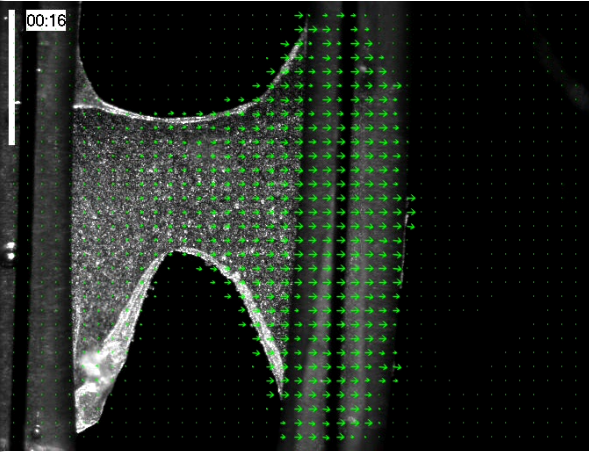
\includegraphics[width=.6\textwidth]{quiver}
  \caption{Vector flow depicted on top of the video frame}
  \label{fig:quiver}
\end{figure}

In order to aid the visualisation of the vector field of the real world data, and therefore assess the qualitative accuracy of the optical flow algorithms, the vectors calculated from the optical flow methods are drawn on top of each frame of the video. The method used is similar to the MATLAB function \verb|quiver| in that it automatically scales the arrows depending on the magnitude of the vector. An example of the output can be seen in figure~\ref{fig:quiver}.

\begin{figure}[htbp!]
  \centering
  \begin{subfigure}[b]{0.45\textwidth}
    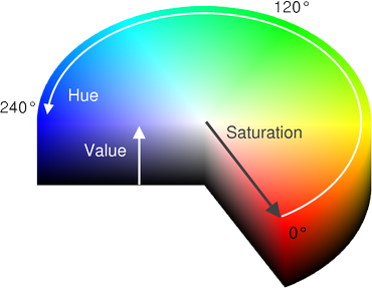
\includegraphics[width=\textwidth]{HSV}
    \caption{Mapping of vectors to HSV colour space}
    \label{fig:hsv}
  \end{subfigure}
  \begin{subfigure}[b]{0.45\textwidth}
    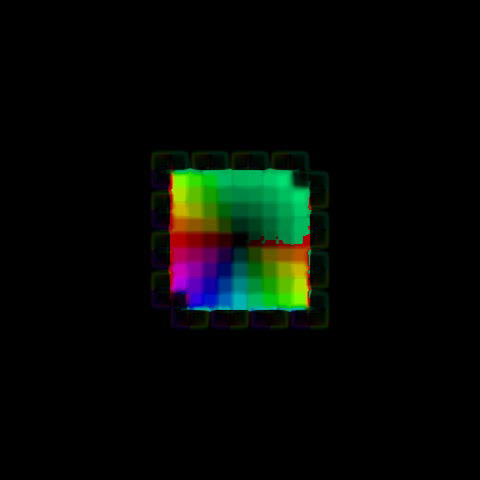
\includegraphics[width=\textwidth]{colour}
    \caption{Colour mapping of a scaling}
    \label{fig:colourmap}
  \end{subfigure}
  \caption{Mapping the vector field to the HSV colour space}
  \label{fig:colour}
\end{figure}

The vector field can also be represented using a colour map. This is achieved by converting the Cartesian vector coordinates into polar coordinates which are then mapped onto the HSV colour space as: Hue = Angle, Saturation = 255, Value = Magnitude. This can be seen in figure~\ref{fig:colour} which depicts the colour mapping of the scaling operation from the artificial dataset. This visualisation method is very useful to gain a quick insight into the apparent motion of the object being observed, without having to further process the vector field from the optical flow algorithm. It should be noted that while this colour mapping is possible for all optical flow algorithms, it is most effective for dense optical flow algorithms. Therefore the Lucas-Kanade algorithm will be required to track all points to achieve a similar output to that of the Farnebäck and SimpleFlow algorithms.

\section{Mechanical Testing}

One of the other goals of this project was the integrate with other projects in the OpenLabTools initiative. One such project was a mechanical testing rig designed and built by Josie Hughes. It allows for tensile testing of materials, and is based around the Arduino, an open-source electronics prototyping platform. Therefore two programs were authored in order to demonstrate online and offline processing. The online processing program makes use of the Lucas-Kanade algorithm due to the ability to select points to be tracked, however it also features an automatic point selector which calculates the minimal eigenvalue of gradient matrices for corner detection. The help text for the online processing program is as follows

\begin{verbatim}
Hot keys:
ESC - quit the program
r - auto-initialize tracking
c - delete all the points
n - switch the "night" mode on/off
To add/remove a feature point click it
\end{verbatim}

Night mode only shows the vector arrows of the flow field over a black background, in an effort to make the optical flow of the points being tracked easier to view. The source code for the online processing program can be seen in full online~\cite{github}

The offline processing program uses the Farnebäck algorithm, and while it is a dense optical flow algorithm, processing time is not as important as we are processing offline. Images for the offline method can be obtained by using the \verb|raspistill| command line program~\cite{raspistill}. The help text for the offline processing program is as follows:

\begin{verbatim}
Usage: ./offline frame1 frame2 output...
\end{verbatim}

The source code for the online processing program can be seen in full online~\cite{github}

In order to test the functionality of the programs, a tensile test of a rubber band was setup. A frame from the testing sequence with the flow field overlaid can be seen in figure~\ref{fig:instron}. This image shows that there is some optical flow occurring in the sequence, however the algorithm, in this example Farnebäck optical flow as this was processed offline, has mostly focused on the motion of the rig holding the rubber band in place. This is most likely due to the high contrast between the rig, and the background. Better framing of the rubber band in the sequence, and a high contrast background behind the mechanical testing rig should eliminate this problem.

\begin{figure}[h]
  \centering
  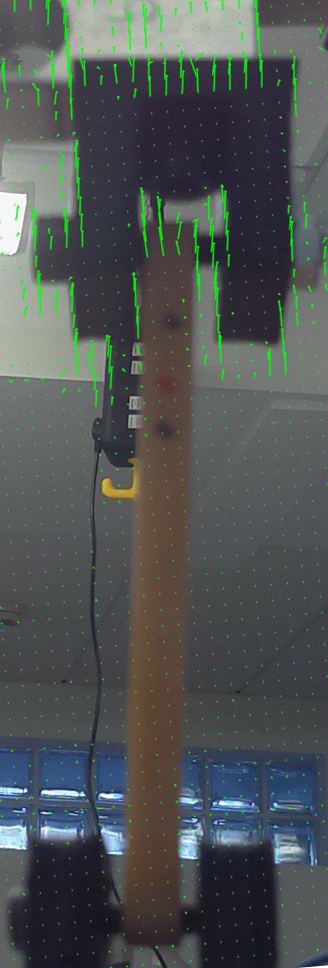
\includegraphics[height=.5\textheight]{output}
  \caption{Tensile test of rubber band}
  \label{fig:instron}
\end{figure}
\chapter{Conclusions}
\label{sec:conclusions}

\ifpdf
    \graphicspath{{Section5/Figs/Raster/}{Section5/Figs/PDF/}{Section5/Figs/}}
\else
    \graphicspath{{Section5/Figs/Vector/}{Section5/Figs/}}
\fi

It has been demonstrated that executing computer vision methods, specifically optical flow algorithms, on the low power and low cost Raspberry Pi system, it is indeed possible to obtain not only high accuracy, but also high speed results within certain requirements. Performing a comparison between Lucas-Kanade, Farnebäck, and SimpleFlow optical flow algorithms for an artificial dataset comprised of individual affine transformations, and forcing Lucas-Kanade optical flow to be a dense optical flow algorithm, there are obvious choices depending on the application. For applications requiring realtime results Farnebäck optical flow appears to be the best choice. For applications which place accuracy above all else, SimpleFlow optical flow shows the best results. Finally, for applications requiring a compromise between accuracy and processing speed, Lucas-Kanade optical flow is a possible choice.

For real world data the results show a slightly different view, mainly due to Lucas-Kanade optical flow being used as a sparse optical flow method instead of being forced to be a dense method. This is another decision that needs to be made when choosing an optical flow method for an application: whether or not a dense flow field is required, or merely flow vectors for key points in the field. Nevertheless, as a true sparse optical flow method, Lucas-Kanade optical flow performs best in terms of processing time per frame, followed by Farnebäck optical flow then SimpleFlow optical flow.

Another aim of this project was to provide a clear set of instructions aimed at undergraduate level. This was achieved early on in the project as many of the tools, such as OpenCV, were used heavily in this project. The instructions can be seen in code listing~\ref{lst:opencv} in Appendix~\ref{sec:appendix} and will soon be found on the OpenLabTools website. In addition, to show the practical applications of optical flow methods in other areas of engineering, a further aim of the project was to integrate with other projects in the OpenLabTools. One such project was a mechanical testing rig designed and built by Josie Hughes, which allows for tensile testing of materials. Using optical flow methods the strain can be measured, and there is recent research which allows the Poisson ratio to be calculated from flow field data from optical flow methods~\cite{chen2013new}. While this project does not explore these avenues, there is certainly scope for doing so using the robust tool set used in this project.

There is scope for extension in several areas of this project. Within the comparison only individual affine transformations were explored, whereas combinations of affine transformations are not. Single affine transformations are less likely to occur in real world data, than arbitrary affine transformations, therefore it may be worth investigating. The tools used to analyse the artificial dataset was written to support, not only single affine transformations, or even arbitrary affine transformations, but projective transformations too. Therefore it should be relatively simple to pursue this area of research. Better visualisation of the vector field is also another possible extension. Currently the vector field can be visualised using vector arrows, or as a colour mapping to HSV colour space, however showing the curl or the divergence of the vector field may also be a useful tool. If the vector field represents the flow velocity of a moving fluid, then the curl is the circulation density of the fluid and the divergence measures the magnitude of a vector field's source or sink at a given point.

% ********************************** Back Matter *******************************
% Backmatter should be commented out, if you are using appendices after References
%\backmatter 

% ********************************** Bibliography ******************************
\begin{spacing}{0.9}

% To use the conventional natbib style referencing
% Bibliography style previews: http://nodonn.tipido.net/bibstyle.php

%\bibliographystyle{apalike}
\bibliographystyle{plainnat} % use this to have URLs listed in References

\cleardoublepage
\bibliography{References/references} % Path to your References.bib file


% If you would like to use BibLaTeX for your references, pass `custombib' as 
% an option in the document class. The location of 'reference.bib' should be 
% specified in the preamble.tex file in the custombib section. 
% Comment out the lines related to natbib above and uncomment the following line.

% \printbibliography[heading=bibintoc, title={References}]


\end{spacing}

% ********************************** Appendices ********************************

\begin{appendices} % Using appendices environment for more functunality

% ******************************* Thesis Appendix A ********************************
\chapter{How to install \LaTeX} 

\section*{Windows OS}

\subsection*{TeXLive package - full version}
\begin{enumerate}
\item	Download the TeXLive ISO (2.2GB) from\\
\href{https://www.tug.org/texlive/}{https://www.tug.org/texlive/}
\item	Download WinCDEmu (if you don't have a virtual drive) from \\
\href{http://wincdemu.sysprogs.org/download/}{http://wincdemu.sysprogs.org/download/}
\item	To install Windows CD Emulator follow the instructions at\\
\href{http://wincdemu.sysprogs.org/tutorials/install/}{http://wincdemu.sysprogs.org/tutorials/install/}
\item	Right click the iso and mount it using the WinCDEmu as shown in \\
\href{http://wincdemu.sysprogs.org/tutorials/mount/}{http://wincdemu.sysprogs.org/tutorials/mount/}
\item	Open your virtual drive and run setup.pl
\end{enumerate}

or

\subsection*{Basic MikTeX - TeX distribution}
\begin{enumerate}
\item	Download Basic-MiK\TeX (32bit or 64bit) from\\
\href{http://miktex.org/download}{http://miktex.org/download}
\item	Run the installer 
\item	To add a new package go to Start >> All Programs >> MikTex >> Maintenance (Admin) and choose Package Manager
\item	Select or search for packages to install
\end{enumerate}

\subsection*{TexStudio - Tex Editor}
\begin{enumerate}
\item	Download TexStudio from\\
\href{http://texstudio.sourceforge.net/\#downloads}{http://texstudio.sourceforge.net/\#downloads} 
\item	Run the installer
\end{enumerate}

\section*{Mac OS X}
\subsection*{MacTeX - TeX distribution}
\begin{enumerate}
\item	Download the file from\\
\href{https://www.tug.org/mactex/}{https://www.tug.org/mactex/}
\item	Extract and double click to run the installer. It does the entire configuration, sit back and relax.
\end{enumerate}

\subsection*{TexStudio - Tex Editor}
\begin{enumerate}
\item	Download TexStudio from\\
\href{http://texstudio.sourceforge.net/\#downloads}{http://texstudio.sourceforge.net/\#downloads} 
\item	Extract and Start
\end{enumerate}


\section*{Unix/Linux}
\subsection*{TeXLive - TeX distribution}
\subsubsection*{Getting the distribution:}
\begin{enumerate}
\item	TexLive can be downloaded from\\
\href{http://www.tug.org/texlive/acquire-netinstall.html}{http://www.tug.org/texlive/acquire-netinstall.html}.
\item	TexLive is provided by most operating system you can use (rpm,apt-get or yum) to get TexLive distributions
\end{enumerate}

\subsubsection*{Installation}
\begin{enumerate}
\item	Mount the ISO file in the mnt directory
\begin{verbatim}
mount -t iso9660 -o ro,loop,noauto /your/texlive####.iso /mnt
\end{verbatim}

\item	Install wget on your OS (use rpm, apt-get or yum install)
\item	Run the installer script install-tl.
\begin{verbatim}
	cd /your/download/directory
	./install-tl
\end{verbatim}
\item	Enter command `i' for installation

\item	Post-Installation configuration:\\
\href{http://www.tug.org/texlive/doc/texlive-en/texlive-en.html\#x1-320003.4.1}{http://www.tug.org/texlive/doc/texlive-en/texlive-en.html\#x1-320003.4.1} 
\item	Set the path for the directory of TexLive binaries in your .bashrc file
\end{enumerate}

\subsubsection*{For 32Bit OS}
For Bourne-compatible shells such as bash, and using Intel x86 GNU/Linux and a default directory setup as an example, the file to edit might be \begin{verbatim}
edit $~/.bashrc file and add following lines
PATH=/usr/local/texlive/2011/bin/i386-linux:$PATH; 
export PATH 
MANPATH=/usr/local/texlive/2011/texmf/doc/man:$MANPATH;
export MANPATH 
INFOPATH=/usr/local/texlive/2011/texmf/doc/info:$INFOPATH;
export INFOPATH
\end{verbatim}
\subsubsection*{For 64Bit}
\begin{verbatim}
edit $~/.bashrc file and add following lines
PATH=/usr/local/texlive/2011/bin/x86_64-linux:$PATH;
export PATH 
MANPATH=/usr/local/texlive/2011/texmf/doc/man:$MANPATH;
export MANPATH 
INFOPATH=/usr/local/texlive/2011/texmf/doc/info:$INFOPATH;
export INFOPATH

\end{verbatim}



%\subsection{Installing directly using Linux packages} 
\subsubsection*{Fedora/RedHat/CENTOS:}
\begin{verbatim} 
sudo yum install texlive 
sudo yum install psutils 
\end{verbatim}


\subsubsection*{SUSE:}
\begin{verbatim}
sudo zypper install texlive
\end{verbatim}


\subsubsection*{Debian/Ubuntu:}
\begin{verbatim} 
sudo apt-get install texlive texlive-latex-extra 
sudo apt-get install psutils
\end{verbatim}

% ******************************* Thesis Appendix B ********************************

\chapter{Installing the CUED Class file}

\LaTeX.cls files can be accessed system-wide when they are placed in the
<texmf>/tex/latex directory, where <texmf> is the root directory of the user’s \TeX installation. On systems that have a local texmf tree (<texmflocal>), which
may be named ``texmf-local'' or ``localtexmf'', it may be advisable to install packages in <texmflocal>, rather than <texmf> as the contents of the former, unlike that of the latter, are preserved after the \LaTeX system is reinstalled and/or upgraded.

It is recommended that the user create a subdirectory <texmf>/tex/latex/CUED for all CUED related \LaTeX class and package files. On some \LaTeX systems, the directory look-up tables will need to be refreshed after making additions or deletions to the system files. For \TeX Live systems this is accomplished via executing ``texhash'' as root. MIK\TeX users can run ``initexmf -u'' to accomplish the same thing.

Users not willing or able to install the files system-wide can install them in their personal directories, but will then have to provide the path (full or relative) in addition to the filename when referring to them in \LaTeX.


% ******************************* Thesis Appendix C ********************************
\chapter{Results}
\label{sec:appendix3}

\ifpdf
  \graphicspath{{Appendix3/Figs/Raster/}{Appendix3/Figs/PDF/}{Appendix3/Figs/}}
\else
  \graphicspath{{Appendix3/Figs/Vector/}{Appendix3/Figs/}}
\fi

\begin{table}[htbp]
  \centering
  \begin{tabular}{r|rr|rr|rr}
    \toprule
    & \multicolumn{2}{c}{Lucas-Kanade} & \multicolumn{2}{c}{Farnebäck} & \multicolumn{2}{c}{SimpleFlow} \\
    \midrule
    Subsampling & Time (s) & Error & Time (s) & Error & Time (s) & Error \\
    \midrule
    1     & 94.67 & 1.94E+00 & 6.62  & 2.10E+00 & 267.59 & 2.11E+00 \\
    2     & 23.80 & 9.83E-01 & 1.64  & 1.06E+00 & 66.83 & 1.06E+00 \\
    4     & 6.09  & 6.31E-01 & 0.44  & 5.35E-01 & 16.80 & 5.32E-01 \\
    8     & 1.69  & 5.01E-01 & 0.10  & 3.44E-01 & 4.29  & 2.70E-01 \\
    16    & 0.56  & 4.14E-01 & 0.02  & 3.61E-01 & 1.08  & 1.40E-01 \\
    \bottomrule
  \end{tabular}
  \caption{Rotation}
  \label{tab:rotation}
\end{table}

\begin{table}[htbp]
  \centering
  \begin{tabular}{r|rr|rr|rr}
    \toprule
    & \multicolumn{2}{c}{Lucas-Kanade} & \multicolumn{2}{c}{Farnebäck} & \multicolumn{2}{c}{SimpleFlow} \\
    \midrule
    Subsampling & Time (s) & Error & Time (s) & Error & Time (s) & Error \\
    \midrule
    1 & 103.12 & 1.27E+02 & 6.77  & 1.20E+02 & 273.10 & 1.21E+02 \\
    2 & 26.02 & 6.66E+01 & 1.62  & 5.97E+01 & 67.99 & 6.05E+01 \\
    4 & 6.75  & 3.66E+01 & 0.39  & 2.99E+01 & 17.05 & 3.05E+01 \\
    8 & 1.82  & 2.29E+01 & 0.08  & 1.47E+01 & 4.24  & 1.55E+01 \\
    16 & 0.60  & 1.34E+01 & 0.02  & 6.96E+00 & 1.09  & 8.00E+00 \\
    \bottomrule
  \end{tabular}
  \caption{Scale}
  \label{tab:scale}
\end{table}

\begin{table}[htbp]
  \centering
  \begin{tabular}{r|rr|rr|rr}
    \toprule
    & \multicolumn{2}{c}{Lucas-Kanade} & \multicolumn{2}{c}{Farnebäck} & \multicolumn{2}{c}{SimpleFlow} \\
    \midrule
    Subsampling & Time (s) & Error & Time (s) & Error & Time (s) & Error \\
    \midrule
    1 & 113.71 & 2.70E+00 & 6.69  & 1.12E-01 & 269.52 & 0.00E+00 \\
    2 & 28.57 & 2.69E+00 & 1.61  & 1.00E-01 & 67.25 & 9.00E-02 \\
    4 & 7.40  & 2.71E+00 & 0.40  & 1.72E-01 & 16.88 & 0.00E+00 \\
    8 & 2.02  & 2.62E+00 & 0.09  & 1.80E-01 & 4.24  & 0.00E+00 \\
    16 & 0.64  & 2.94E+00 & 0.02  & 8.97E-01 & 1.08  & 0.00E+00 \\
    \bottomrule
  \end{tabular}
  \caption{Shear}
  \label{tab:shear}
\end{table}


\begin{table}[htbp]
  \centering
  \begin{tabular}{r|rr|rr|rr}
    \toprule
    & \multicolumn{2}{c}{Lucas-Kanade} & \multicolumn{2}{c}{Farnebäck} & \multicolumn{2}{c}{SimpleFlow} \\
    \midrule
    Subsampling & Time (s) & Error & Time (s) & Error & Time (s) & Error \\
    \midrule
    1 & 79.79 & 1.00E+01 & 6.92  & 1.00E+01 & 268.98 & 1.00E+01 \\
    2 & 20.29 & 1.00E+01 & 1.69  & 1.00E+01 & 67.01 & 1.00E+01 \\
    4 & 5.23  & 1.00E+01 & 0.47  & 1.00E+01 & 17.02 & 1.00E+01 \\
    8 & 1.47  & 1.00E+01 & 0.11  & 1.00E+01 & 4.27  & 1.00E+01 \\
    16 & 0.51  & 1.00E+01 & 0.02  & 1.01E+01 & 1.08  & 1.00E+01 \\
    \bottomrule
  \end{tabular}
  \caption{Translate}
  \label{tab:translate}
\end{table}

\end{appendices}

% *************************************** Index ********************************
\printthesisindex % If index is present

\end{document}
